\documentclass{SCIS2020cn}
%%%%%%%%%%%%%%%%%%%%%%%%%%%%%%%%%%%%%%%%%%%%%%%%%%%%%%%
%%% 作者附加的定义
%%% 常用环境已经加载好, 不需要重复加载
%%%%%%%%%%%%%%%%%%%%%%%%%%%%%%%%%%%%%%%%%%%%%%%%%%%%%%%
\usepackage{xspace}
\usepackage{ulem}
\newcommand{\ve}{\overline{\nu}_e}
\newcommand{\MADGRAPH}{\textsc{MadGraph}\xspace}
\newcommand{\MCATNLO}{\textsc{mc@nlo}\xspace}
\newcommand{\MGvATNLO}{$\MADGRAPH${}5\_a\MCATNLO}
\newcommand{\POWHEG}{{\textsc{powheg}}\xspace}
\newcommand{\PYTHIA}{{\textsc{pythia}}\xspace}
\newcommand{\SHERPA}{{\textsc{sherpa}}\xspace}
\newcommand{\GEANTfour}{{\textsc{Geant4}}\xspace}
\newcommand{\Wboson}{\text{W}}
\newcommand{\Zboson}{\text{Z}}
\newcommand{\Hboson}{\text{H}}
\newcommand{\mass}{\text{m}}
\newcommand{\add}{\textcolor{blue}}
\newcommand{\rmv}[1]{\textcolor{red}{\sout{#1}}}
\defaultfontfeatures[TeX Gyre Termes]
{
  Extension      = .otf ,
  UprightFont    = texgyretermes-regular,
  BoldFont       = texgyretermes-bold,
  ItalicFont     = texgyretermes-italic,
  BoldItalicFont = texgyretermes-bolditalic,
}
\setmainfont{TeX Gyre Termes}

% 列表的行距
\usepackage{enumitem}
\setenumerate[1]{itemsep=0pt,partopsep=0pt,parsep=\parskip,topsep=5pt}
\setitemize[1]{itemsep=0pt,partopsep=0pt,parsep=\parskip,topsep=5pt}
\setdescription{itemsep=0pt,partopsep=0pt,parsep=\parskip,topsep=5pt}

%%%%%%%%%%%%%%%%%%%%%%%%%%%%%%%%%%%%%%%%%%%%%%%%%%%%%%%
%%% 开始
%%%%%%%%%%%%%%%%%%%%%%%%%%%%%%%%%%%%%%%%%%%%%%%%%%%%%%%
\begin{document}

%%%%%%%%%%%%%%%%%%%%%%%%%%%%%%%%%%%%%%%%%%%%%%%%%%%%%%%
%%% 作者不需要修改此处信息
\ArticleType{评述}
%\SpecialTopic{}
%\Luntan{中国科学院学部\quad 科学与技术前沿论坛}
\Year{2020}
\Vol{50}
\No{1}
\BeginPage{1}
\DOI{}
\ReceiveDate{}
\ReviseDate{}
\AcceptDate{}
\OnlineDate{}
%%%%%%%%%%%%%%%%%%%%%%%%%%%%%%%%%%%%%%%%%%%%%%%%%%%%%%%

\title{大型强子对撞机上CMS实验矢量玻色子散射的物理研究}{大型强子对撞机上CMS实验矢量玻色子散射的物理研究}

\entitle{Vector Boson Scattering from the CMS experiment at the Large Hadron Collider}{Vector Boson Scattering from the CMS experiment at the Large Hadron Collider}

\author[]{卢梦}{{meng.lu@cern.ch}}
\author[]{戴自霖}{{daizl@pku.edu.cn}}
\author[]{黄迁明}{}
\author[]{安莹}{}
\author[]{肖杰}{}
\author[]{彭靖}{}
% TODO: 「喆」楷体无法显示
\author[]{关吉吉}{}
\author[]{冒亚军}{}
\author[]{班勇}{}
\author[]{李强}{{qliphy0@pku.edu.cn}}

\enauthor[]{LU Meng}{{meng.lu@cern.ch}}
\enauthor[]{DAI ZiLin}{{daizl@pku.edu.cn}}
\enauthor[]{Huang QianMing}{}
\enauthor[]{An Ying}{}
\enauthor[]{Xiao Jie}{}
\enauthor[]{Peng Jing}{}
\enauthor[]{Guan Zhe}{}
\enauthor[]{Mao YaJun}{}
\enauthor[]{Ban Yong}{}
\enauthor[]{LI Qiang}{{qliphy0@pku.edu.cn}}

\address[]{北京大学物理学院核物理与核技术国家重点实验室, 北京 100871}

\enaddress[]{School of Physics, State Key laboratory of Nuclear Physics and Technology, Beijing {\rm 100871}}

\Foundation{科技部国家重点研发计划(编号2018YFA0403900)、国家自然科学基金(编号: 11661141008)资助项目}

\AuthorMark{卢梦等}

\AuthorCitation{卢梦, 戴自霖, 黄迁明, 等}
\enAuthorCitation{Lu M, Dai Z L, Huang Q M, et al}

%\comment{\dag~同等贡献}
%\encomment{\dag~Equal contribution}

\abstract{在标准模型中, Higgs 场结合电弱对称自发破缺机制赋予基本粒子质量, 同时 Higgs 玻色子的存在保证了有质量的矢量玻色子散射过程的幺正性不被破坏. 矢量玻色子散射过程除了对验证 Higgs机制具有重要意义, 还可以作为寻找标准模型之外的新物理的探针. 本文将在简要回顾标准模型中 Higgs 理论之后, 详细地介绍从基于蒙特卡洛样本对同号WW散射的早期研究, 到利用CMS实验一期和二期取数对矢量玻色子散射过程的寻找和利用该过程对超出标准模型的新物理进行的研究, 以及近期CMS实验组实现的LHC上第一次对矢量玻色子散射过程的极化部分的测量.}

\enabstract{Triggered by the electroweak symmetry spontaneous breaking, the Higgs boson gives mass to fundamental particles, and ensures the unitarity safety of the vector boson scattering. Not only crucial to test Higgs mechanism, vector boson scattering can also be used to probe new physics beyond the standard model. In this paper, after a brief introduction of the standard model Higgs theory, we present a detailed review on the vector boson scattering research, from the early study on the same charged WW based on Monte Carlo samples, the searches for vector boson scattering and studies on the beyond standard model physics using data collected by CMS experiment during Run1 in 2012 and Run2 from 2016 to 2018, to the first measurement on the polarized vector boson scattering which is performed recently.}

\keywords{标准模型, Higgs玻色子, 矢量玻色子散射, 新物理}

\enkeywords{standard model, higgs boson, vector boson scattering, new physics}

% TODO: PACS font
\pacs{12.15.−y, 14.70.Fm, 14.70.Hp, 14.70.Bh}

\maketitle

\section{引言}
2010年, 位于瑞士与法国边境上的大型强子对撞机\upcite{1}(Large Hadron Collider, LHC)正式启动, 并成功实现了质心能量为7 TeV的质子对撞. 两年后的2012年, LHC上的ATLAS \upcite{2,3}实验以5.9倍标准偏差发现了质量为126.0$\pm$0.6 GeV的新粒子\upcite{4}, CMS\upcite{5,6}实验以5.0倍标准偏差发现了质量为125.3$\pm$0.7 GeV的新粒子\upcite{7}. 两个独立实验都以超过5倍标准偏差发现了新粒子, 那么如何确定该粒子是否为标准模型中的Higgs粒子呢? 标准模型中预言了Higgs粒子在不同质量下的衰变模式, 如图 \ref{fig:1}所示. 

\begin{figure}[!t]
\centering
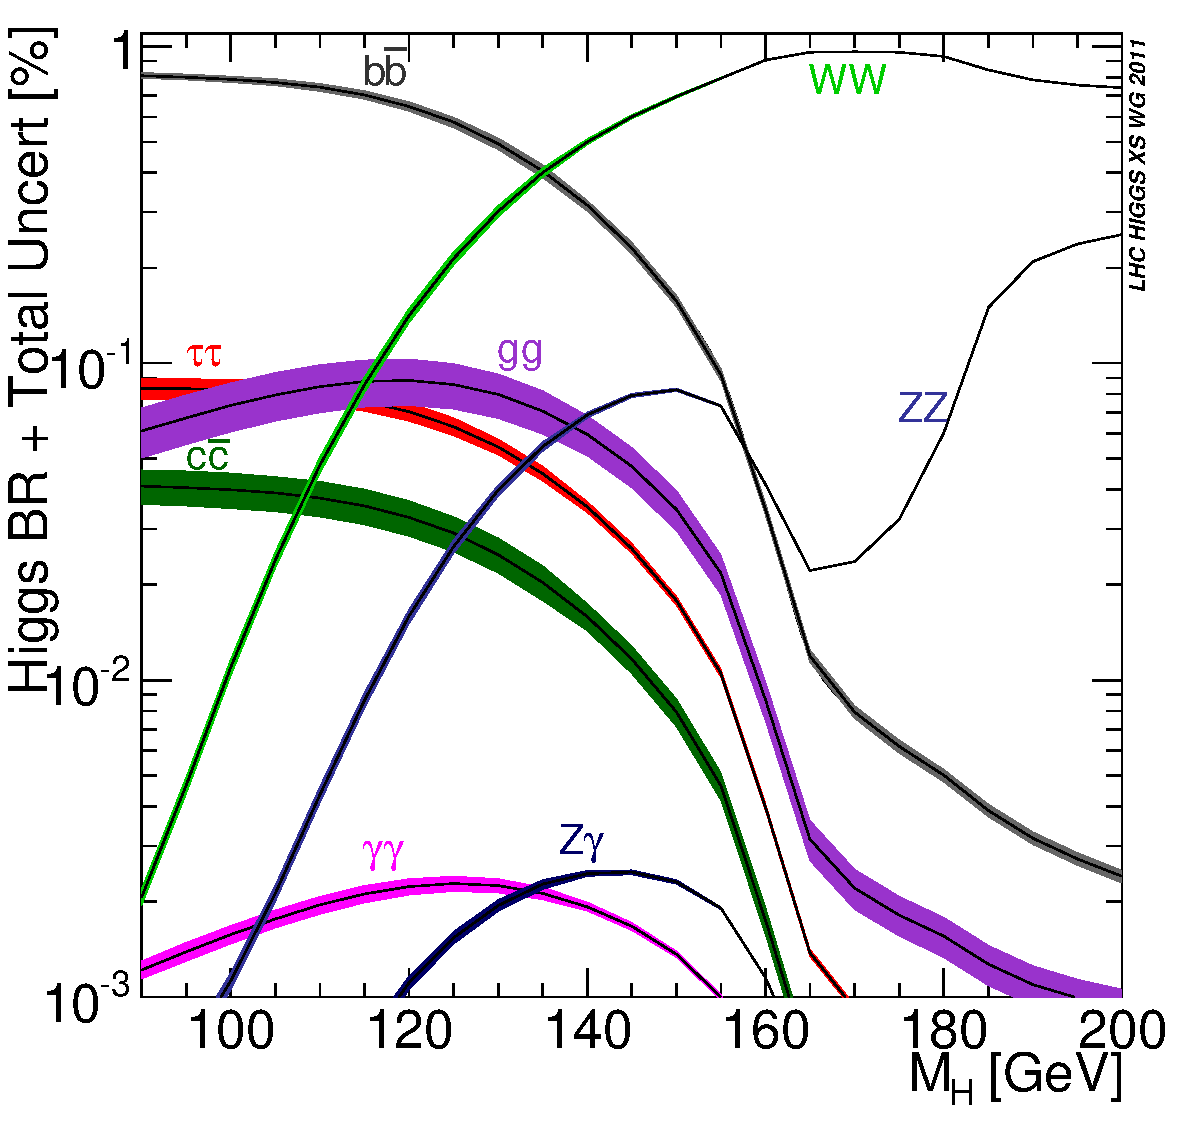
\includegraphics[width=2.72396in]{Figure-1.pdf}
\cnenfigcaption{标准模型Higgs粒子的衰变分支比及其误差\upcite{8}}{SM Higgs Boson decay branching ratios and their uncertainties\upcite{8}}
\label{fig:1}
\end{figure}

通过测量新粒子衰变的各种末态, 并与标准模型进行对比, 就可以知道这个粒子是否为我们寻找的Higgs粒子. 利用7 TeV和8 TeV的对撞数据, CMS实验组测量了新粒子的五个衰变道: 

\begin{enumerate}
\def\labelenumi{\arabic{enumi}.}
\item H $\rightarrow$ $\gamma$$\gamma$,
\item H $\rightarrow$ ZZ,
\item H $\rightarrow$ W\textsuperscript{+}W\textsuperscript{-},
\item H $\rightarrow$ $\tau$\textsuperscript{+}$\tau$\textsuperscript{-},
\item H $\rightarrow$ $b\overline{b}$.
\end{enumerate}

这五个道的信号强度$\sigma/\sigma_{SM}$如图 \ref{fig:2} 所示, 最终的综合信号强度为0.87$\pm$0.23. 与此同时,ATLAS实验组发现了质量为126 GeV的新粒子,综合各个道的综合信号强度为1.4$\pm$0.3. 两个实验独立的发现了质量为125 GeV附近的新粒子,且该新粒子的衰变分支比与标准模型中预言的质量为125 GeV的Higgs粒子的衰变分支比在误差范围内符合,因此这个新粒子很大可能就是人们一直在寻找的Higgs粒子。在这之后, 通过更大统计量以及更高能量的对撞数据得到的结果也确认这一结论\upcite{64,65,66,67}. 

\begin{figure}[ht!]
\centering
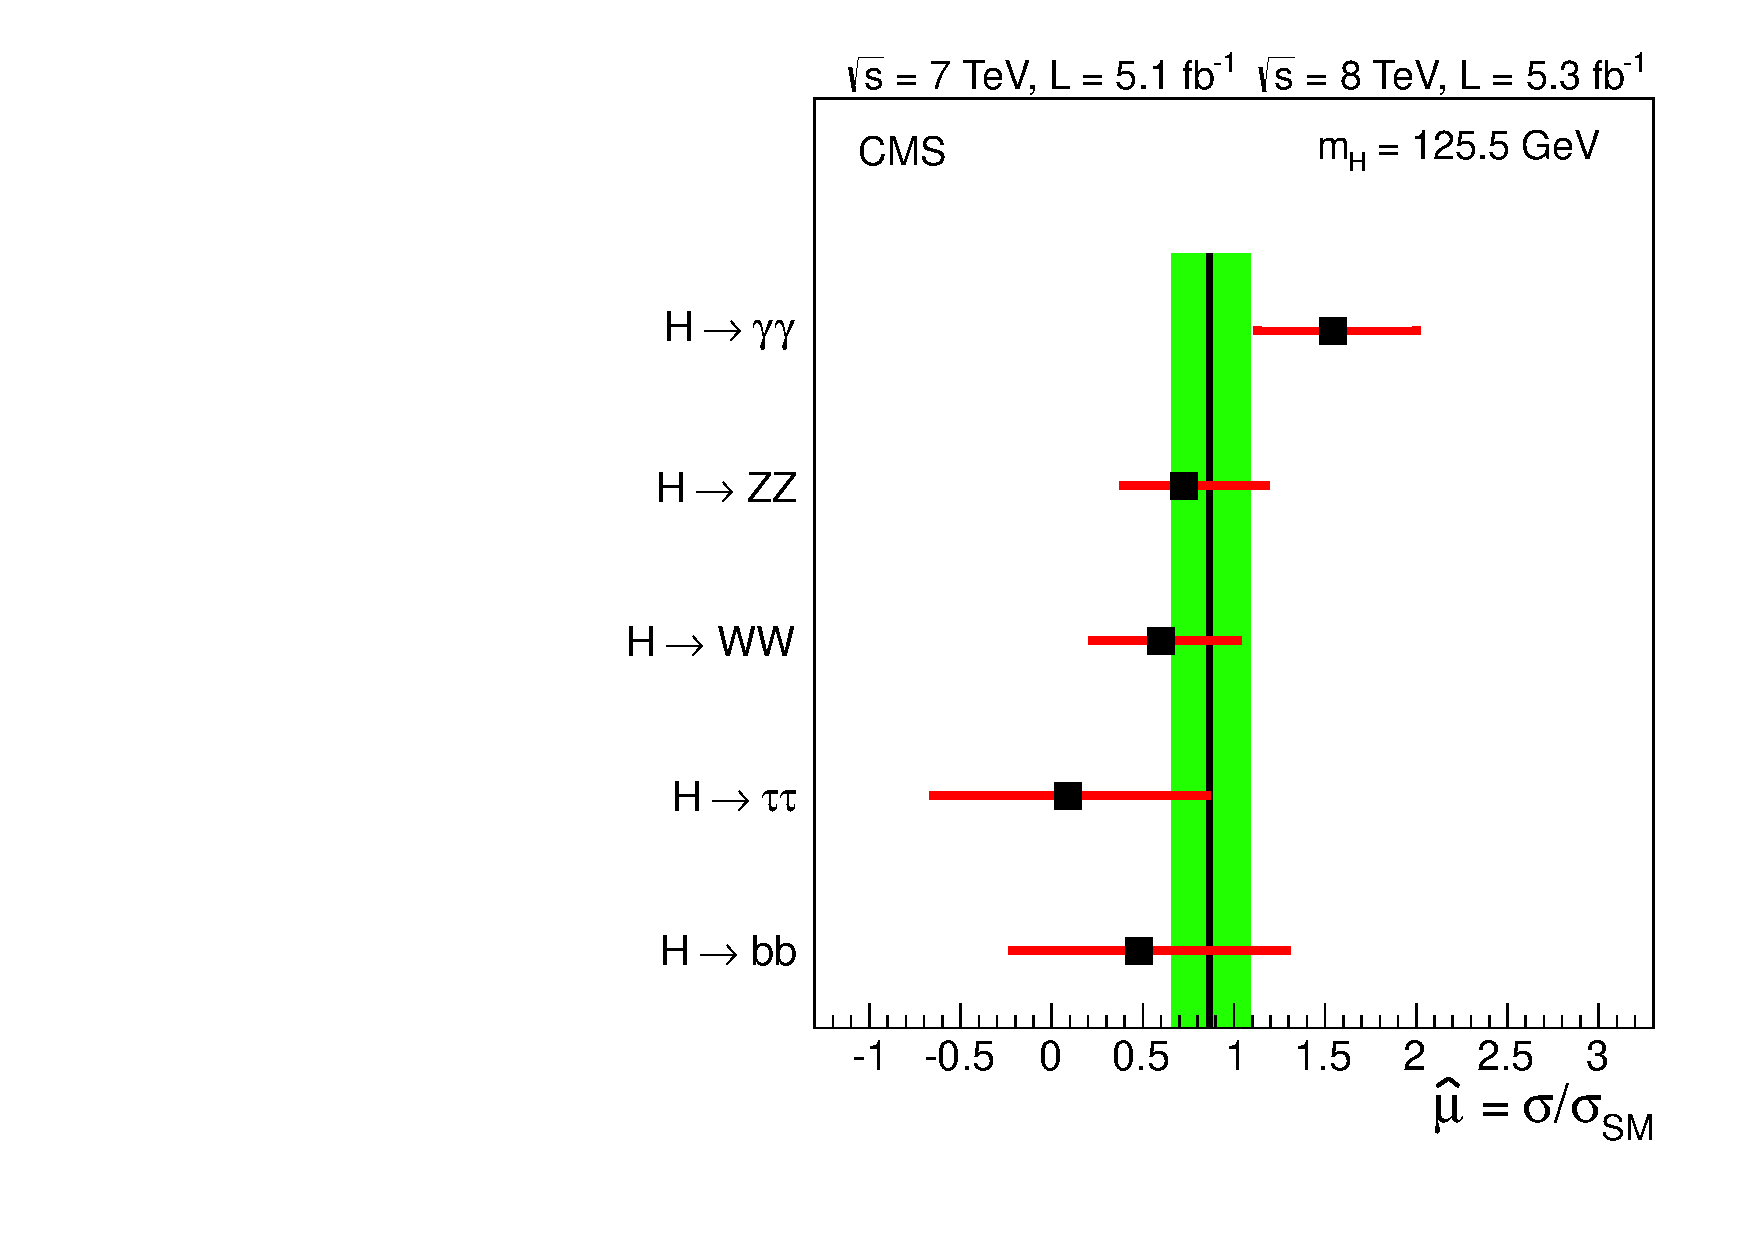
\includegraphics[width=2.65104in]{Figure-2.pdf}
\cnenfigcaption{CMS利用7 TeV和8 TeV数据得到的各个衰变道的信号强度, 综合所有道后的信号强度和误差(分别为黑点和红线)为$0.87\pm0.23$, 在误差范围内与标准模型符合\upcite{63}}{The combination of 7 TeV and 8 TeV signal strengths of individual decay modes and their uncertainties (black points and red lines). The vertical green bar centered with black line is the overall signal strength $0.87\pm0.23$. The overall signal strength is consistent with SM within uncertainty\upcite{63}}
\label{fig:2}
\end{figure}

Higgs粒子被发现之后, 人们已经找到了标准模型预言的所有粒子. 为什么Higgs粒子如此重要, 以致于人们称之为上帝粒子呢? 一部分原因是因为它是标准模型中最后一个被找到的粒子, 它的发现补全了标准模型, 这是粒子物理学的一个里程碑. 另一方面, Higgs玻色子的质量是标准模型中的一个自由参量, 这大大加剧了寻找难度. 不过, 最重要的原因在于Higgs场\upcite{9,10,11,12}通过Higgs玻色子赋予了基本粒子质量. 

在试图创建描述弱相互作用的理论时, 由于局域对称性的要求, 物理学家们在描述粒子运动的拉氏量中引入了规范场, 但是这种规范场对应的玻色子质量为零, 这与只观测到一种零质量矢量玻色子——光子的事实相悖, 因此如何赋予这些零质量玻色子质量成为难题. 另一方面, Nambu等人在研究超导现象时发现了对称性自发破缺 (spontaneous symmetry breaking, SSB) 现象\upcite{13,14}, 这一现象应用在粒子物理中将会导致零质量Goldstone玻色子. 在1964年, Higgs等人将SSB机制与局域对称性相结合, 发现规范场论中的长程力变成了短程力, 即零质量的规范玻色子通过与Goldstone玻色子结合形成了有质量的规范玻色子, 这为后来的电弱统一理论\upcite{15,16,17}奠定了基础. Higgs场经过SSB后剩余的物理自由度的激发态为Higgs玻色子.

我们知道, 光子只有两个偏振自由度. 在没有引入SSB机制之前, 规范场的玻色子为零质量, 因此它们和光子一样, 也只有两个偏振自由度. 而通过SSB机制, 这些玻色子获得了质量. 规范玻色子``吃掉'' Goldstone玻色子, Goldstone玻色子成为其第三偏振分量, 即纵向偏振, 这表明矢量规范玻色子的纵向分量与SSB机制直接相关. 在Higgs玻色子被发现之后, 除了研究Higgs玻色子本身的性质, 比如质量的精确测量、与玻色子以及费米子之间的耦合是否与标准模型符合、自耦合强度等等\upcite{18,19}, 与有质量矢量玻色子的纵向极化相关的测量也极大地吸引着人们的兴趣. 

对纵向分量进行测量的黄金过程为矢量玻色子散射过程(Vector Boson Scattering, VBS), 该过程的典型费曼图如图 \ref{fig:3} 所示. 两个入射的部分子分别辐射出一个矢量玻色子, 这两个矢量玻色子之间发生散射得到另外两个矢量玻色子. 在探测器中, 入射部分子辐射之后的剩余部分将经历强子簇射(也包括一些电磁簇射), 形成两个喷注. VBS过程有以下几个特点: 

\begin{itemize}
\item 末态两个喷注为背对背方向, 二者之间的赝快度差值很大;
\item 两个喷注的不变质量可以达到TeV量级;
\item 由于玻色子之间没有色荷流存在, 因此两个喷注之间的强相互作用活动被很大程度地压低.
\end{itemize}

\begin{figure}[ht!]
\centering
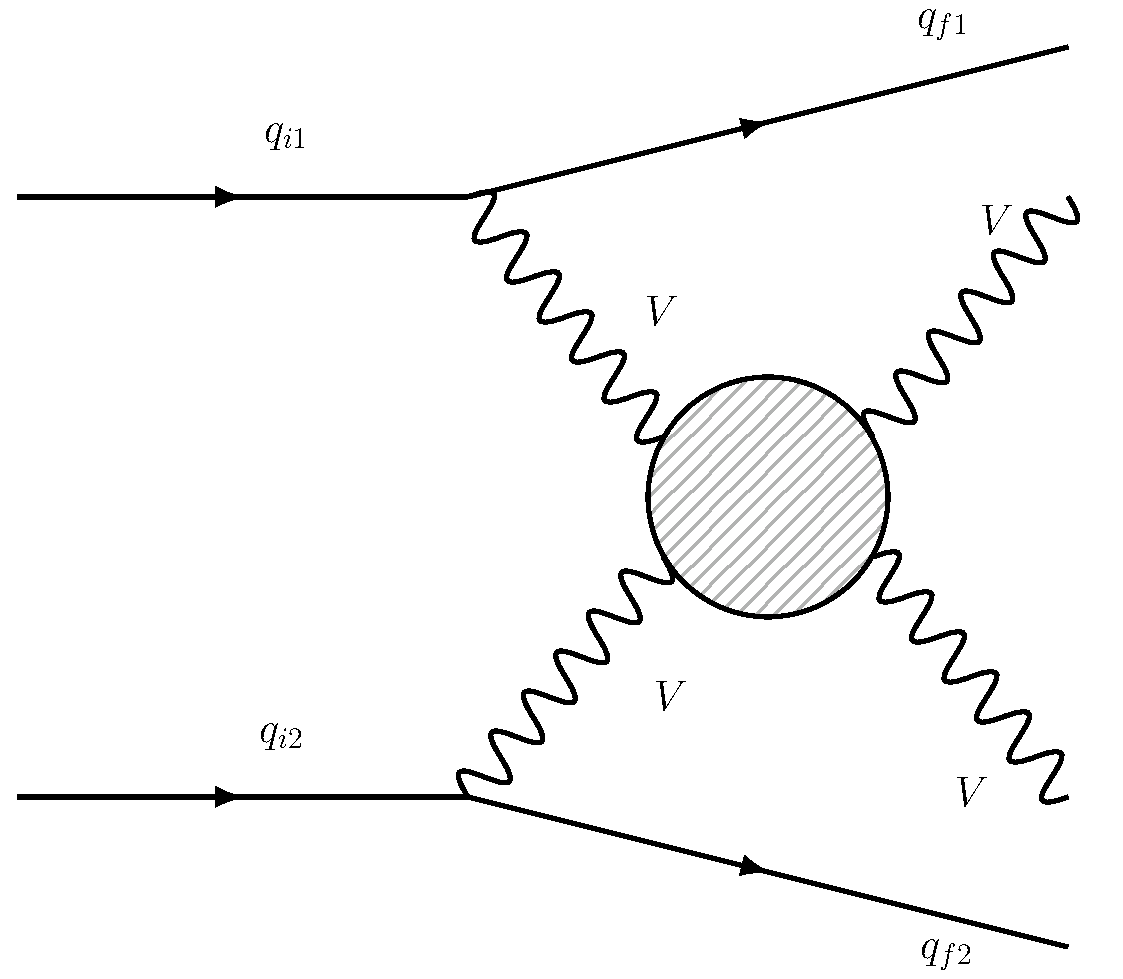
\includegraphics[width=2.65104in]{Figure-3.pdf}
\cnenfigcaption{VBS过程费曼图}{Typical Feynman diagram of VBS process}
\label{fig:3}
\end{figure}

正如前文所述, VBS过程的重要性在于其包含的纵向分量之间的散射. 在Higgs粒子被发现之前, 就已经有相关的工作对矢量玻色子纵向分量散射过程进行了研究\upcite{20}. 如图 \ref{fig:4} \upcite{21}所示, 在同电荷W玻色子的散射过程中, 横向极化之间的散射截面加上横向与纵向极化之间的散射截面并不会随着质心能量的增加而发散. 但是对于纵向极化之间的散射, 若是没有Higgs粒子存在, 其散射截面将会随着质心系能量的增加而发散, 带来幺正性的破坏, 这在量子理论中是不可接受的. 从图 \ref{fig:4} 中看出, 不同质量的Higgs粒子对于纵向极化散射过程的影响也是不一样的, 因此在Higgs玻色子被发现后, 检验含标准模型Higgs玻色子贡献的VBS过程的高能行为是否与实验观测相一致将会是对标准模型的又一次考验. 

\begin{figure}[ht!]
\centering
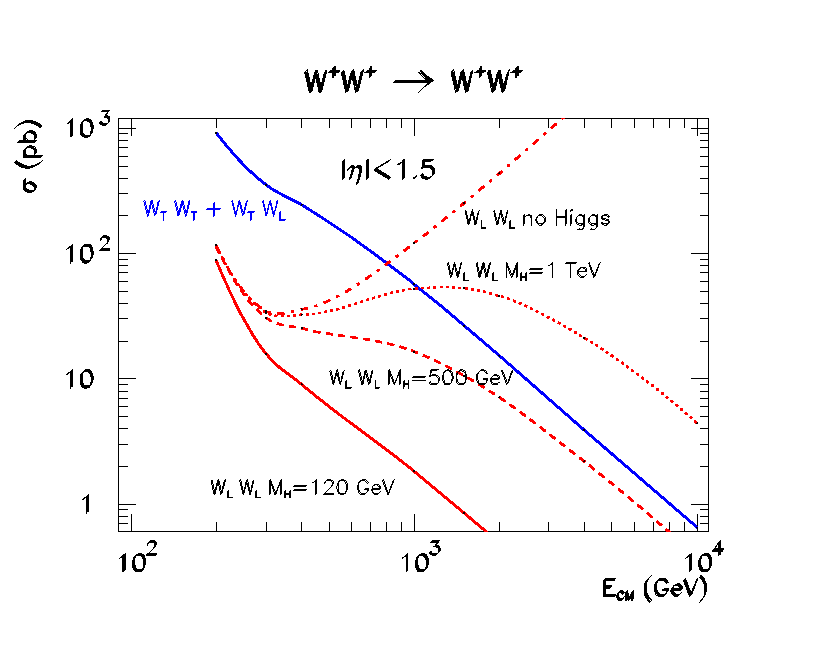
\includegraphics[width=3in]{Figure-4.pdf}
\cnenfigcaption{在不同Higgs粒子质量以及不存在Higgs粒子的假设下,同号WW散射过程不同极化部分的截面随对撞质心能量的变化图\upcite{21}}{The total $\Wboson^+\Wboson^+$ scattering cross sections as a function of the center of mass
energy for different final (and initial) state polarizations and for different Higgs masses,
including the limiting Higgsless case\upcite{21}}
\label{fig:4}
\end{figure}

VBS过程除了对SSB机制的研究有重要意义, 还可以指引人们探寻标准模型之外的物理. 长久以来, 寻找标准模型之外的物理是人们的梦想. 对于新物理的寻找可以分为两个方向. 第一种为直接寻找标准模型中不存在的新粒子, 例如超对称理论\upcite{22}预言存在超对称粒子. 第二种为寻找标准模型粒子之间的反常耦合, 有效场理论\upcite{23,24,25}就属于这一类. 有效场理论的拉氏量如下: 

\begin{align}
\mathcal{L}=\mathcal{L}_{S M}+\sum_i\left[\frac{c_{i}}{\Lambda^{2}} \mathcal{O}_{i}^{(6)}+\frac{e_{i}}{\Lambda^{4}} \mathcal{O}_{i}^{(8)}+\cdots\right]
\end{align}

其中$\mathcal{L}_{S M}$代表标准模型的拉氏量, 其量纲为质量的四次方. $\mathcal{O}_{i}^{(d)}$为具有质量$d$次方量纲的算符. 对于本文涉及的矢量玻色子散射, 这些高阶算符包括玻色子之间的反常相互作用项, 例如$d=6$时对应的是三规范玻色子顶点, $d=8$时对应的是四规范玻色子顶点等等. $c_i,e_i$为无量纲系数, $\Lambda$为新物理对应的能标, 在实际应用中, 可以将$\Lambda$看作远大于现在能达到的能量尺度. 有效场理论是与具体模型无关的, 它利用标准模型中已有的场量来进行构建, 所有在标准模型对称变换下保持不变的算符都可以成为它的一部分. 原则上, 所有$d>4$的算符都可以包括进来, 但是当$d=5$时, 对应的算符负责产生中微子的Majorana质量, 将会破坏轻子数守恒. 其他的奇数次方项算符会破坏轻子数或者重子数守恒, 因此对于规范玻色子之间的相互作用只考虑偶数阶的算符. 

VBS过程可以根据散射出来的两个玻色子进行分类: 

\begin{enumerate}
\def\labelenumi{\arabic{enumi}.}
\item VBS WW (同号或者异号W,\ ssWW/osWW),
\item VBS WZ,
\item VBS ZZ,
\item VBS $\Zboson\gamma$,
\item VBS $\Wboson\gamma$.
\end{enumerate}

除此之外, 还可以根据玻色子的衰变模式进一步将这些过程分为轻子衰变道和强子衰变道. 不过强子衰变道的分析主要集中于反常耦合的测量, 这里介绍的工作将只包括轻子衰变模式的VBS过程. 在上述的过程中, VBS WW/WZ/ZZ这些有质量玻色子的过程可以进行纵向极化散射的幺正性研究, 这对于理解SSB机制具有重要意义. VBS $\Zboson\gamma$/$\Wboson\gamma$则因为光子没有纵向极化分量, 因此与SSB机制不直接相关. 

对VBS过程的测量在LHC一期取数期间就已经开始, 其中CMS在$\Zboson\gamma$道得到了VBS的第一个3倍标准偏差的结果\upcite{26}. 而利用二期(2016年)取数的分析中, CMS在5倍标准偏差水平观测到了同号WW\upcite{27}以及$\Wboson\gamma$\upcite{28}道, 其中同号WW散射是LHC上第一个在5倍标准偏差水平被确立的VBS过程. 

\begin{table}[!t]
\cnentablecaption{CMS实验利用一期取数得到的VBS过程中三个道的结果, 其中VBS $\Zboson\gamma$得到了CMS上第一个VBS的3倍标准偏差发现}{Results of three VBS channels using Run1 data, while $\Zboson\gamma$ is the first observed $3\sigma$ evidence of VBS process in CMS}
\label{tab:1}
\footnotesize
\tabcolsep 39pt %space between two columns. 用于调整列间距
\begin{tabular*}{\textwidth}{cccc}
\toprule
& 预期显著度 & 观测显著度 &
数据亮度/fb\textsuperscript{-1} \\ \hline
VBS ssWW & 3.1$\sigma$ & 2.0$\sigma$ & 19.4 \\
VBS $\Zboson\gamma$ & 2.1$\sigma$ & 3.0$\sigma$ & 19.7 \\
VBS $\Wboson\gamma$ & 1.5$\sigma$ & 2.7$\sigma$ & 19.7 \\ 
\bottomrule
\end{tabular*}
\end{table}

\begin{table}[!t]
\cnentablecaption{CMS实验利用二期取数得到的VBS过程中五个道的结果, 其中VBS ssWW得到了LHC上第一个VBS的超过5倍标准偏差发现. 表格中括号内的值为结合一期取数之后的结果}{Results of five VBS channels using Run2 data, while ssWW is the first discovery of VBS process in LHC. The numbers in parentheses are the results combining Run1 and Run2 data}
\label{tab:2}
\footnotesize
\tabcolsep 39pt %space between two columns. 用于调整列间距
\begin{tabular*}{\textwidth}{cccc}
\toprule
& 预期显著度 & 观测显著度 &
数据亮度/fb\textsuperscript{-1} \\ \hline
VBS ssWW & 5.7$\sigma$ & 5.5$\sigma$ & 35.9\\
VBS WZ & 2.5$\sigma$ & 2.2$\sigma$ & 35.9\\
VBS ZZ & 1.6$\sigma$ & 2.7$\sigma$ & 35.9\\
VBS $\Zboson\gamma$ & 5.2(5.5)$\sigma$ & 3.9(4.7)$\sigma$ & 35.9(55.6)\\
VBS $\Wboson\gamma$ & 4.6(4.8)$\sigma$ & 4.9(5.3)$\sigma$ & 35.9(55.6)\\
\bottomrule
\end{tabular*}
\end{table}

除了表 \ref{tab:1}、表 \ref{tab:2} 中的结果外, 我们还将详细介绍早期利用蒙特卡洛样本进行的ssWW的研究, 以及近期对于纵向极化散射的研究, 其中纵向极化的研究包括了分别基于纯蒙特卡洛样本以及基于CMS取数的几项工作. 

\section{同号WW散射的早期蒙特卡洛研究\upcite{29}}

由于WW散射过程在研究标准模型电弱对称性自发破缺中的重要性, 在Higgs玻色子被发现之前就已经有相关的工作对该过程进行了基于蒙特卡洛的研究. 这项工作研究了同号WW衰变到两个$\mu$子的末态, 蒙特卡洛样本对应的质心系能量和积分亮度分别为10 TeV和60 fb\textsuperscript{-1}. 

信号过程末态为$qq\mu^{\pm}\nu\mu^{\pm}\nu$, 在树图水平是阶为$\mathcal{O}(\alpha^6_{EW})$的纯电弱过程, 主要本底包括含有QCD顶点的同末态过程(QCD本底), 阶为$\mathcal{O}(\alpha^4_{EW}\alpha^2_s)$. 其他本底包括$t\overline{t} \rightarrow \Wboson^+b\Wboson^-b$, 在这项本底中, 一个$\mu$子来自于W玻色子衰变, 另外一个同号的$\mu$子则来自于底夸克衰变的W玻色子. 因此, 基于同样的原因, 单个顶夸克加上W玻色子的过程也需要考虑. 另外一个主要本底为W+喷注过程, 其中一个$\mu$子来自W, 而另一个$\mu$子则来源于喷注中的长寿命的带电强子(例如$k^{\pm},\pi^{\pm},p^{\pm}$)的误鉴别, 由于该过程的截面非常大, 即使很小的误鉴别率也会带来不可忽略的影响. 除了上述的主要本底, 单顶夸克过程、$t\overline{t}\Wboson$以及双玻色子过程(WW, WZ, ZZ)都纳入了考虑. 

信号过程和QCD本底样本利用PHANTOM\upcite{30,31,32}产生, $t\overline{t}$、W+喷注以及$t\overline{t}\Wboson$等利用$\MADGRAPH$\upcite{33,34,35}产生, 其他本底利用$\PYTHIA$\upcite{36,37}产生. 利用PHANTOM产生的过程对应的为领头阶 (Leading Order, LO) 截面, 利用其他产生子产生的样本对应的为次级领头阶 (Next to Leading Order, NLO) 截面. 所有这些样本的部分子簇射(parton showering)和强子化都通过$\PYTHIA$实现, 喷注的重建也是由$\PYTHIA$实现. 为了模拟探测器对物理对应动力学变量的影响, $\mu$子和喷注的动量根据横动量分辨率做了相应的高斯卷积. 

由于Higgs玻色子质量未知, 其质量应当小于1 TeV, 因此这项工作研究了$\mass_{\Hboson}=200$ GeV和$\mass_{\Hboson}=500$ GeV两种情况. 从图 \ref{fig:5} 可以看出, 虽然不同Higgs质量下两个W玻色子不变质量的分布差别较小, 但Higgs玻色子存在与不存在对比时, 相应分布差别较为明显. 由于末态存在两个中微子, 因此两个W玻色子不能被重建出来, 因此可以转而利用两个$\mu$子的不变质量作为鉴别动力学变量. 

\begin{figure}[ht!]
\centering
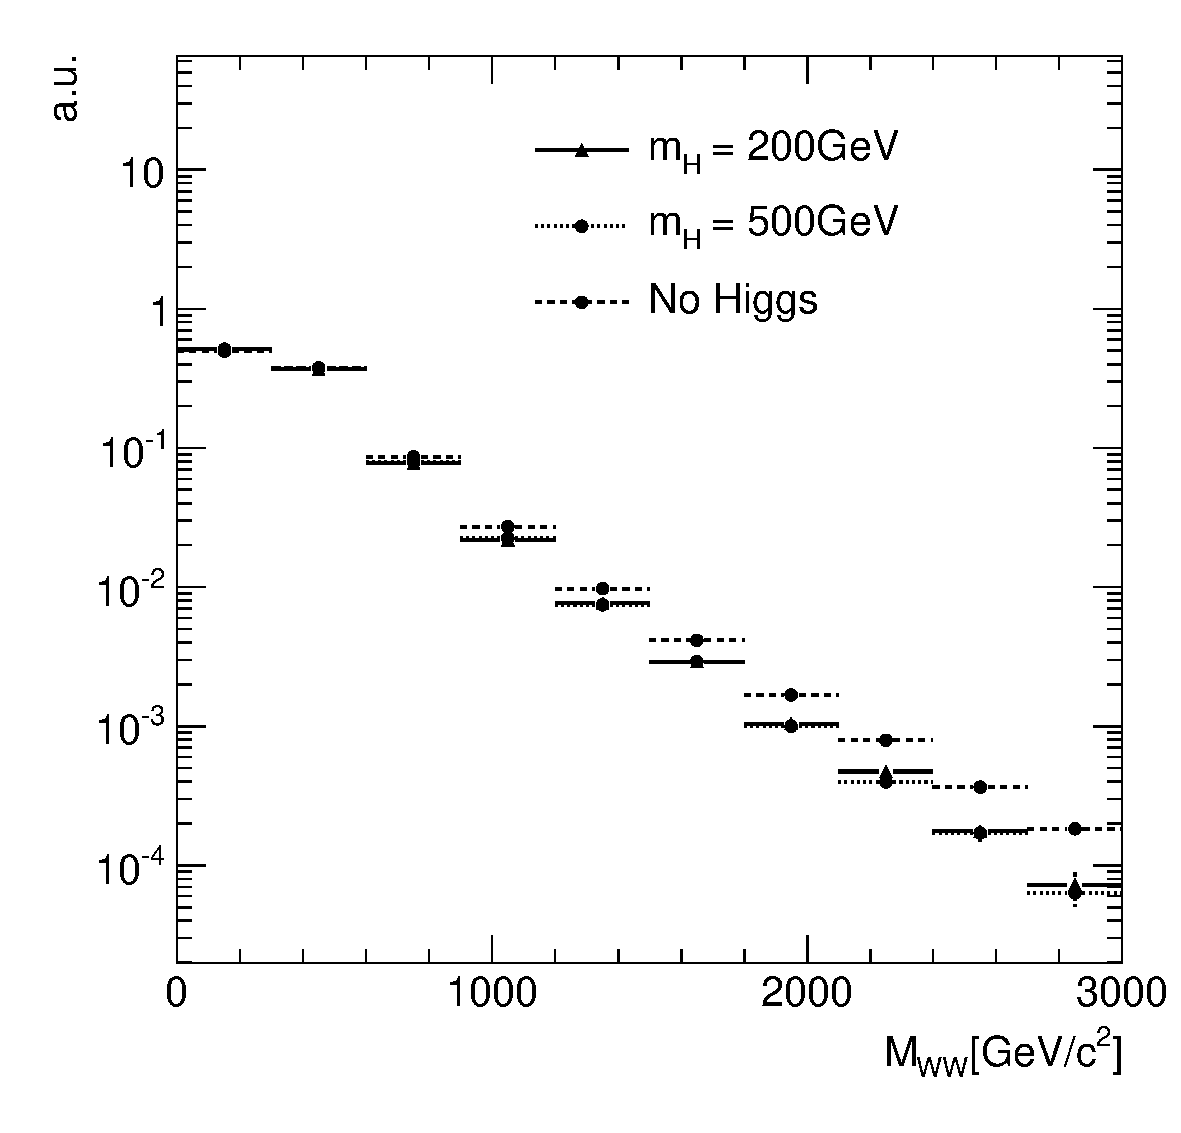
\includegraphics[width=3in]{Figure-5.pdf}
\cnenfigcaption{当Higgs玻色子质量为200 GeV/c\textsuperscript{2}、500 GeV/c\textsuperscript{2}以及Higgs玻色子不存在时双W玻色子不变质量分布\upcite{29}}{$\mass_{\Wboson\Wboson}$ distribution for $\mass_{\Hboson}$ = 200 GeV/c\textsuperscript{2}, $\mass_{\Hboson}$ = 500 GeV/c\textsuperscript{2} and no-Higgs Scenarios. \upcite{29}}
\label{fig:5}
\end{figure}

根据末态具有两个同号$\mu$子的特性, 可以有效的排除末态只有一个$\mu$子或者两个异号$\mu$子的本底. 对于强子被误鉴别为$\mu$子的本底, 这些假$\mu$子的横动量通常较低, 在要求较大的$\mu$子横动量之后也可以有效排除. 除此之外, 根据VBS过程两个喷注的特性, 即要求两个喷注的赝快度差值很大以及具有较大的不变质量, 也可以进一步的排除掉大量的本底. 

利用toy-蒙特卡洛方法, 可以得到不同Higgs玻色子质量情况下的结合似然函数比分布. 图 \ref{fig:6} 对应的是对两个$\mu$子不变质量做筛选, 并且质心系能量为14 TeV, 积分亮度为6 ab\textsuperscript{-1}时, $H_0$假设(Higgs玻色子质量为200 GeV)和$H_1$假设(Higgs玻色子不存在)对应的似然函数比分布. 图 \ref{fig:6} 对应的$H_0$假设和$H_1$假设的区分度为4倍标准偏差.

\begin{figure}[ht!]
\centering
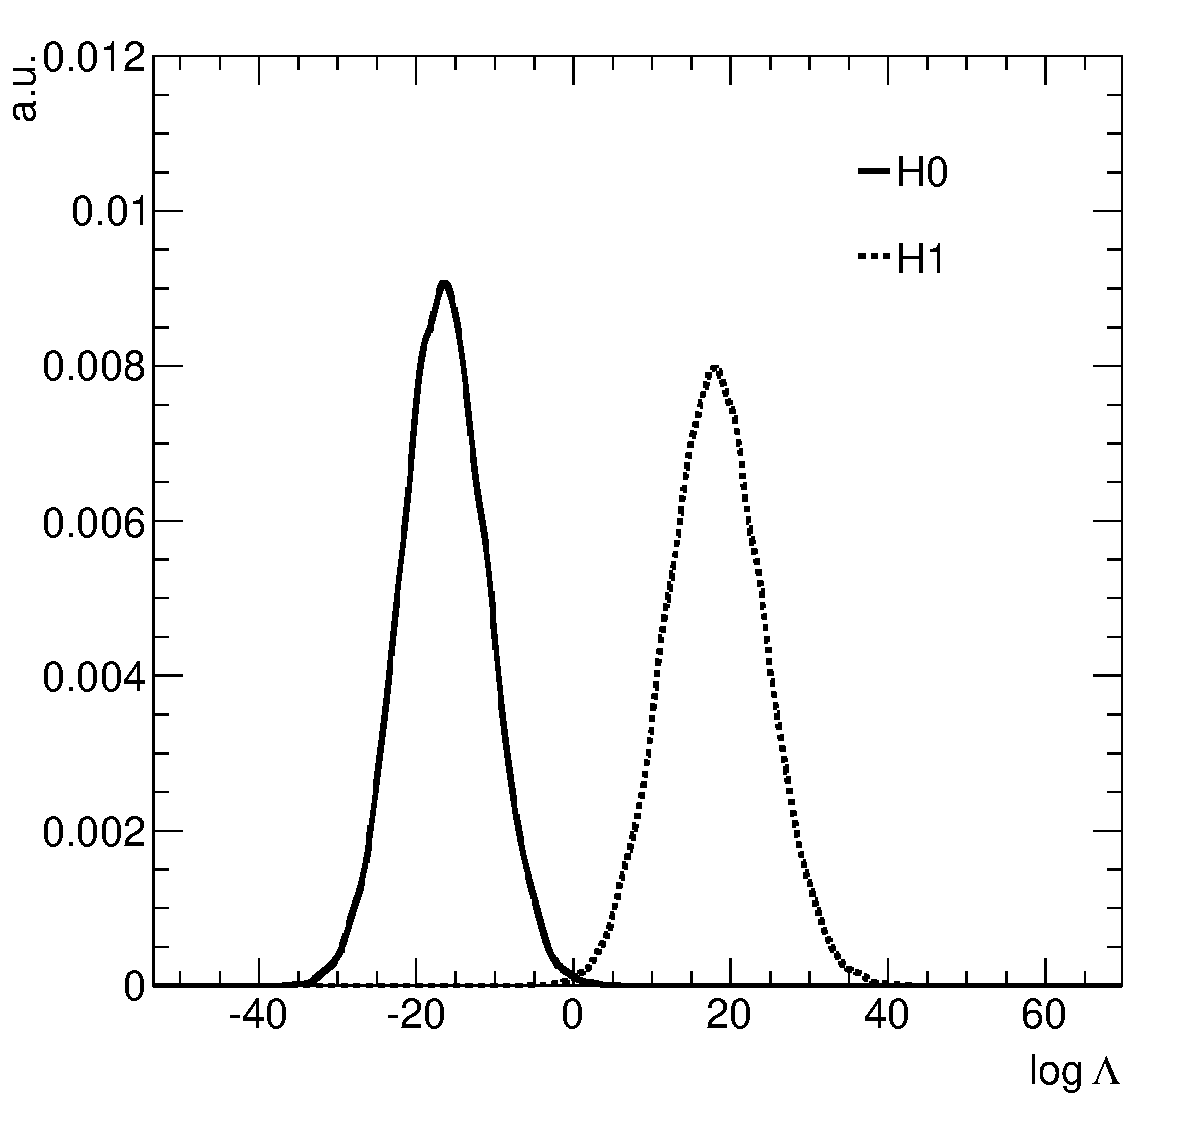
\includegraphics[width=2.78646in]{Figure-6.pdf}
\cnenfigcaption{归一化的似然函数比分布, $H_0$对应Higgs质量为200 GeV, $H_1$对应Higgs玻色子不存在. 结果对应的积分亮度为6 ab\textsuperscript{-1}, 质心系能量为14 TeV\upcite{29}}{Normalized loglikelihood ratio distributions for two hypothesis, $H_0$ corresponds to $\mass_{\Hboson}=200$ GeV, $H_1$ corresponds to no Higgs boson. Results corresponds to an inverse luminosity of 6 ab\textsuperscript{-1} at $\sqrt{s}=14$ TeV\upcite{29}}
\label{fig:6}
\end{figure}

\section{一期数据的VBS分析}
\label{sec:3}

\subsection{同号WW散射}

同号WW散射\upcite{38}分析是CMS上的第一个VBS分析. 这个分析使用的数据由CMS在2012年收集, 对应的积分亮度为19.4 fb\textsuperscript{-1}. 和第二部分介绍的工作类似, 事例选择要求具有两个同号的携带高横动量的轻子、较大的丢失横动量, 以及两个喷注. 

在这个分析中, 根据轻子味道的不同, 末态又可以分为同味道($ee,\mu\mu$)和不同味道($e\mu$). 对于$ee$道, 其中一个电子可能来自于电荷的误判, 即来自于Drell-Yan过程. 通过要求两个电子的不变质量落于Z玻色子的质量窗之外, 并额外要求较大的丢失横动量, 可以有效排除. 包含顶夸克的一类本底($t\overline{t},t\Wboson$), 由于顶夸克会衰变出底夸克, 因此可以通过标记底夸克喷注来有效排除. WZ过程则可以通过要求事例仅仅有两个轻子来排除. 最重要的本底(非瞬发轻子, 即不是来自于硬散射过程的轻子)则是末态的两个轻子中一个来自重夸克衰变或者喷注中的强子的误鉴别, 这类本底可以通过要求两个轻子具有较大的不变质量来排除. 

除了轻子的选择条件, 还要求两个喷注具有较大的赝快度差, 并且具有较大的不变质量. 经过上述所有的事例挑选之后, 15\%的本底来自于WZ, 75\%的本底来自非瞬发轻子本底. 

图 \ref{fig:7} 为两个喷注的不变质量分布, 信号过程包括了纯电弱、QCD以及二者的干涉部分. 其中纯电弱过程占总信号事例的85-90\%, 干涉项占比约为10\%. 将信号分为正电荷和负电荷部分, 并按照图 \ref{fig:7} 所示对喷注不变质量分段, 得到的测量(预期)信号显著度为2.0(3.1)倍标准偏差. 若将信号过程中的QCD部分看作本底, 将电弱部分和干涉部分作为信号, 则测量(预期)信号显著度为1.9(2.9)倍标准偏差. 

\begin{figure}[ht!]
\centering
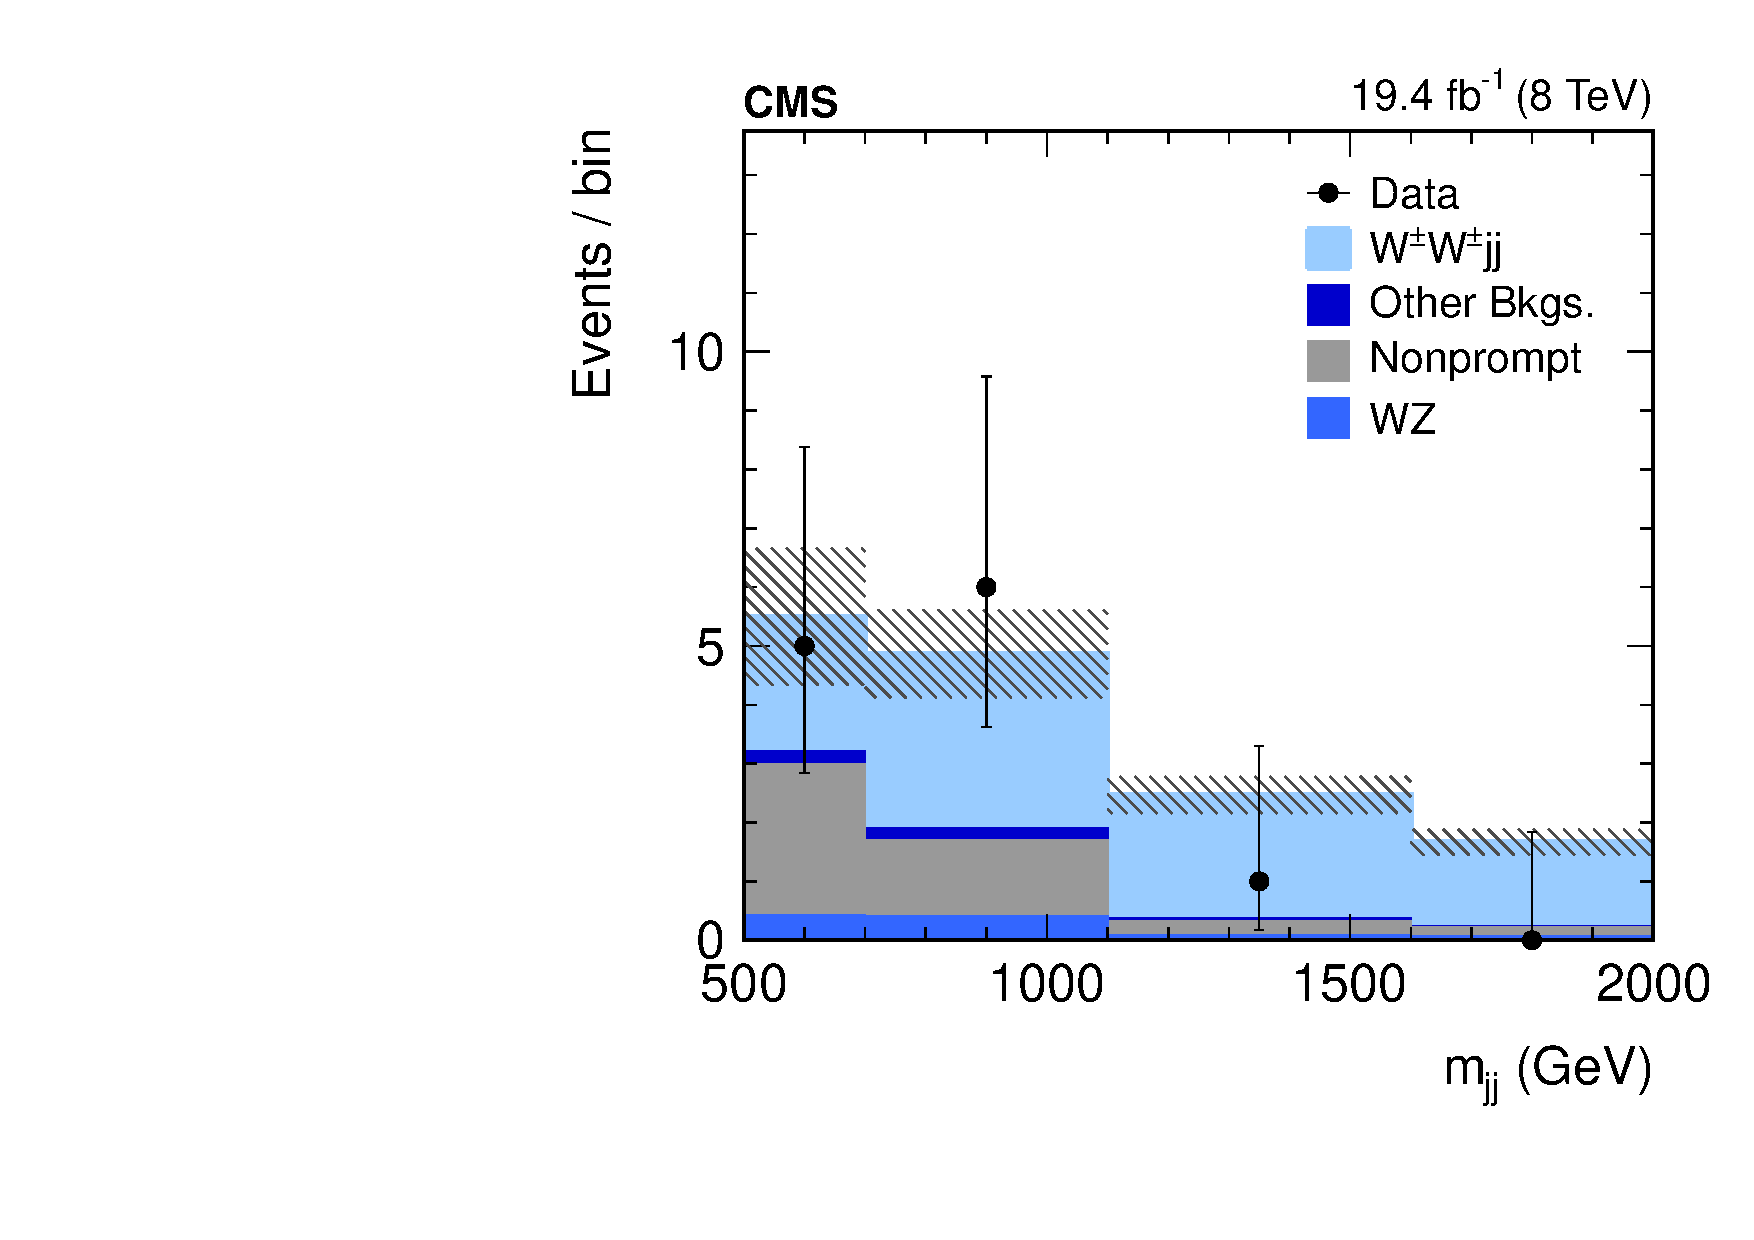
\includegraphics[width=3in]{Figure-7.pdf}
\cnenfigcaption{信号区域两个喷注不变质量分布, 阴影部分包括统计误差和系统误差, 其中WWjj过程包括电弱、QCD以及二者的干涉}{Distribution of invariant mass of two jets in signal region, the hatched bars include statistical and systematic uncertainties. The signal includes EW, QCD and their interference contributions}
\label{fig:7}
\end{figure}

除了标准模型测量部分, 这项工作也对超出标准模型之外的物理做了研究, 包括反常耦合以及$\Hboson^{\pm \pm} \rightarrow \Wboson^{\pm} \Wboson^{\pm}$\upcite{39}的寻找. 分析给出了几项反常耦合算符的上限, 以及不同质量的双电荷Higgs玻色子衰变的截面上限, 如图 \ref{fig:8} 所示. 

\begin{figure}[ht!]
\centering
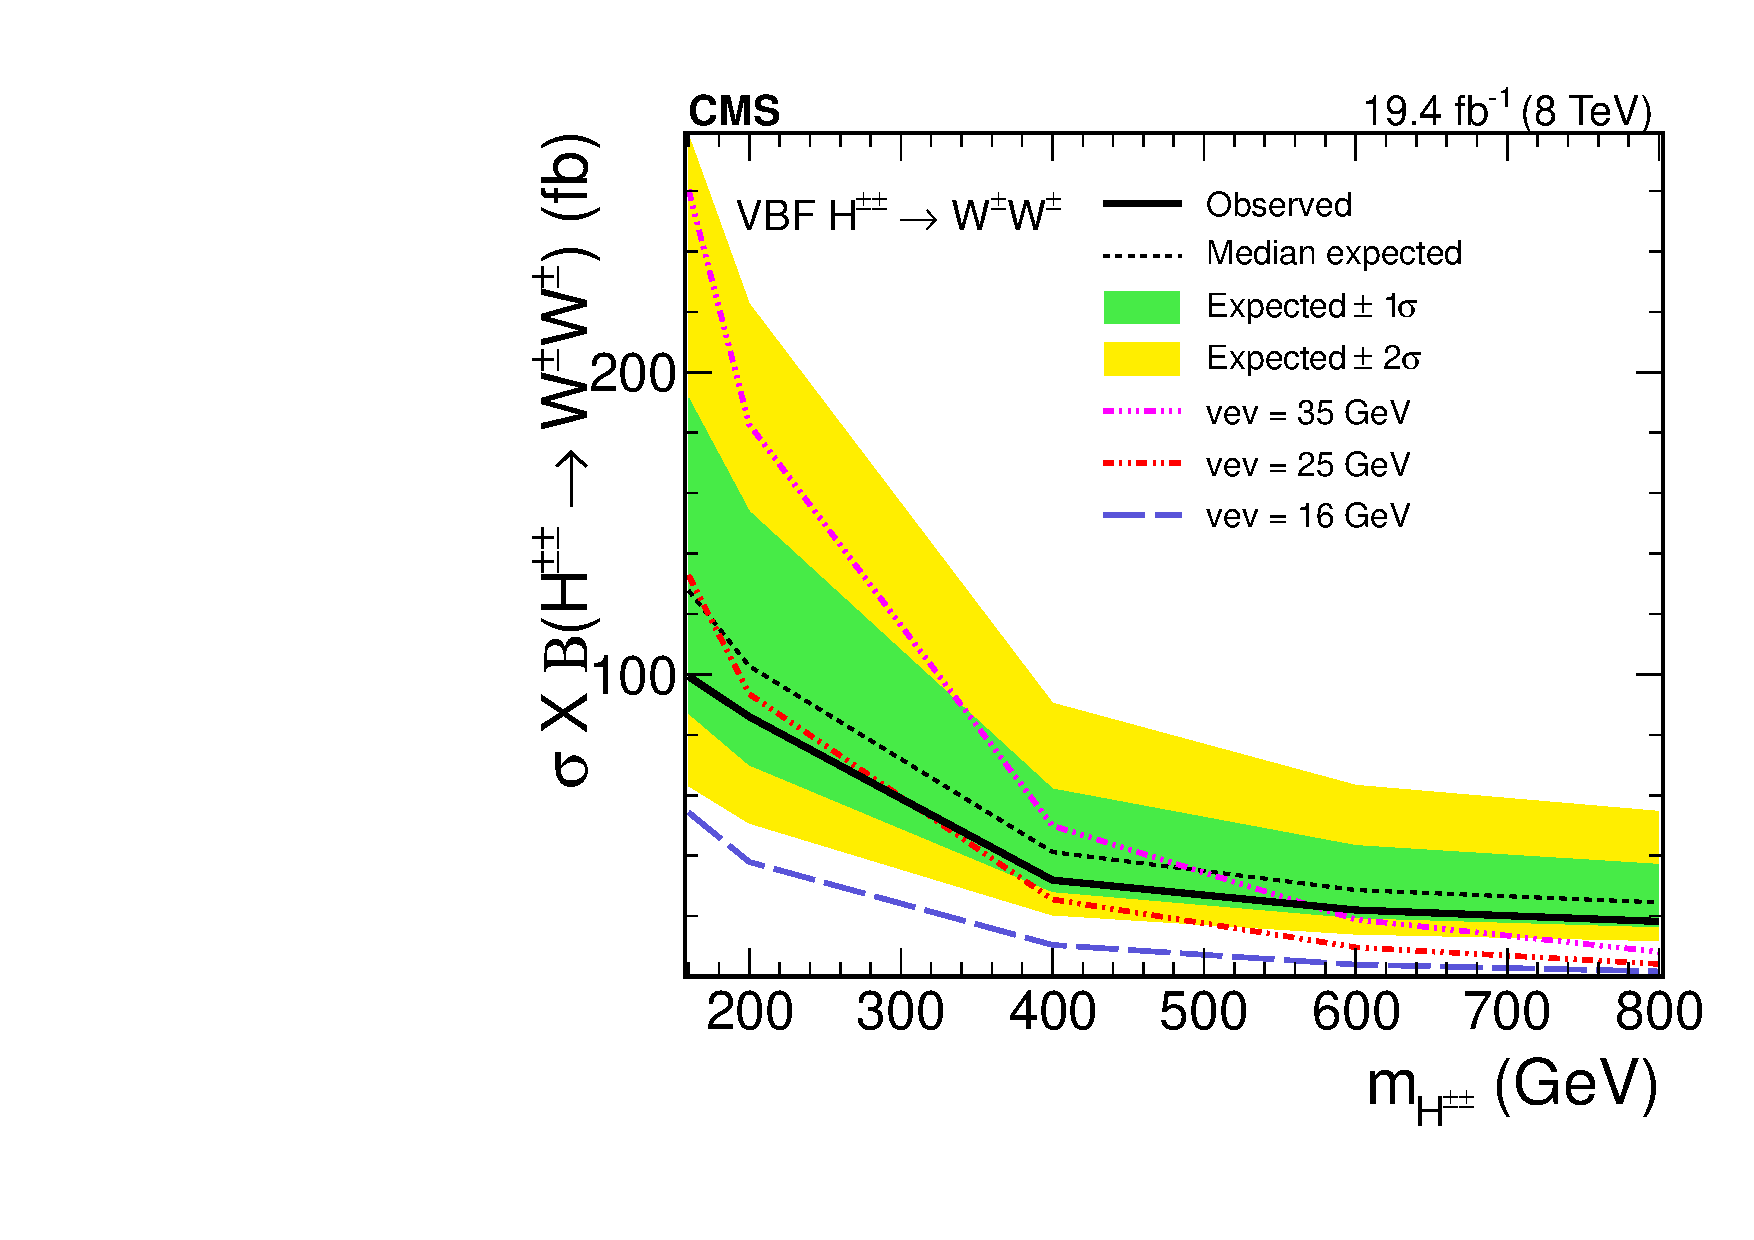
\includegraphics[width=3in]{Figure-8.pdf}
\cnenfigcaption{不同质量下的双电荷Higgs玻色子截面与衰变分支比乘积 $\sigma_{\Hboson^{\pm \pm}} \times B(\Hboson^{\pm \pm} \rightarrow \Wboson^{\pm} \Wboson^{\pm})$ 的上限值, 三种不同真空期望值对应的截面也在图中画出}{Expected and observed 95\% CL upper limits on the cross section times branching
fraction, $\sigma_{\Hboson^{\pm \pm}} \times B(\Hboson^{\pm \pm} \rightarrow \Wboson^{\pm} \Wboson^{\pm})$. Theoretical cross sections for three values of the vacuum expectation value (vev) are overlaid}
\label{fig:8}
\end{figure}

\subsection{$\Wboson\gamma$散射}
\label{sec:3.2}

$\Wboson\gamma$道\upcite{40}的末态为一个轻子、丢失横动量、一个光子以及两个喷注. 分析利用的数据积分亮度为19.7 fb\textsuperscript{-1}. $\Wboson\gamma$道最重要的本底来自于带有QCD顶点的$\Wboson\gamma$过程(以下称为QCD本底)以及非瞬发光子本底. 非瞬发光子主要来自于喷注中的$\pi^0$介子的双光子衰变\upcite{41}. 光子的重建依赖于光子在电磁量能器上的电磁簇射形状、电磁量能器与强子量能器的能量沉积比以及是否存在径迹. 若$\pi^0$介子的横动量比较大, 则来自于$\pi^0$介子的两个光子将会靠的很近, 这会使得它们在电磁量能器上留下的簇射形状和单光子的形状相似, 因此会造成光子的误鉴别. 为了区分这两种相似的簇射形状, 构造所谓的$\sigma_{i \eta i \eta}$变量. $\sigma_{i \eta i \eta}$表示的是簇射在电磁量能器上的集中性, 对于来自硬散射过程的单光子, 其能量更倾向于集中在小范围内, 而来自于中心$\pi^0$介子的双光子的能量则会倾向于分散. 分析通过形状拟合方法, 利用瞬发光子和非瞬发光子的$\sigma_{i \eta i \eta}$的形状去拟合数据, 最终得到数据信号区域的非瞬发光子的比例. 其他的本底的贡献都是利用蒙特卡洛样本来估计, 它们的贡献可以通过一系列的事例挑选条件来压低, 例如通过否决具有一个以上轻子的事例可以有效的排除来自于含有Z玻色子的过程以及双W玻色子的过程. 通过底夸克喷注的标记, 可以有效的压低包含顶夸克的本底过程. VBS过程两个喷注的特性, 即较大的赝快度差以及较大的不变质量, 在保持信号事例的效率时有效的压低本底的贡献. 另外, 对于VBS过程, 两个玻色子的出射方向倾向于背对背, 两个喷注也有这个特性, 因此可以要求整个末态动力学系统在赝快度方向的平衡来压低本底. 

最后, 利用信号区域喷注的不变质量分布, 电弱过程的测量(预期)显著度为2.7(1.5)倍标准偏差. 若把QCD+EW作为信号, 则测量(预期)显著度为7.7(7.5)倍标准偏差. 除了电弱测量, $\Wboson\gamma$道也研究了反常耦合. 由于反常耦合的效应在较为极端的相空间更明显, 因此要求光子的横动量大于200 GeV, 同时利用重建出来的W玻色子的横动量来研究反常耦合对于信号的抬高行为. 结果如图 \ref{fig:9} 所示, 数据和标准模型预期值在误差范围内符合, 因此对反常耦合算符的强度做了限制. 

\begin{figure}[ht!]
\centering
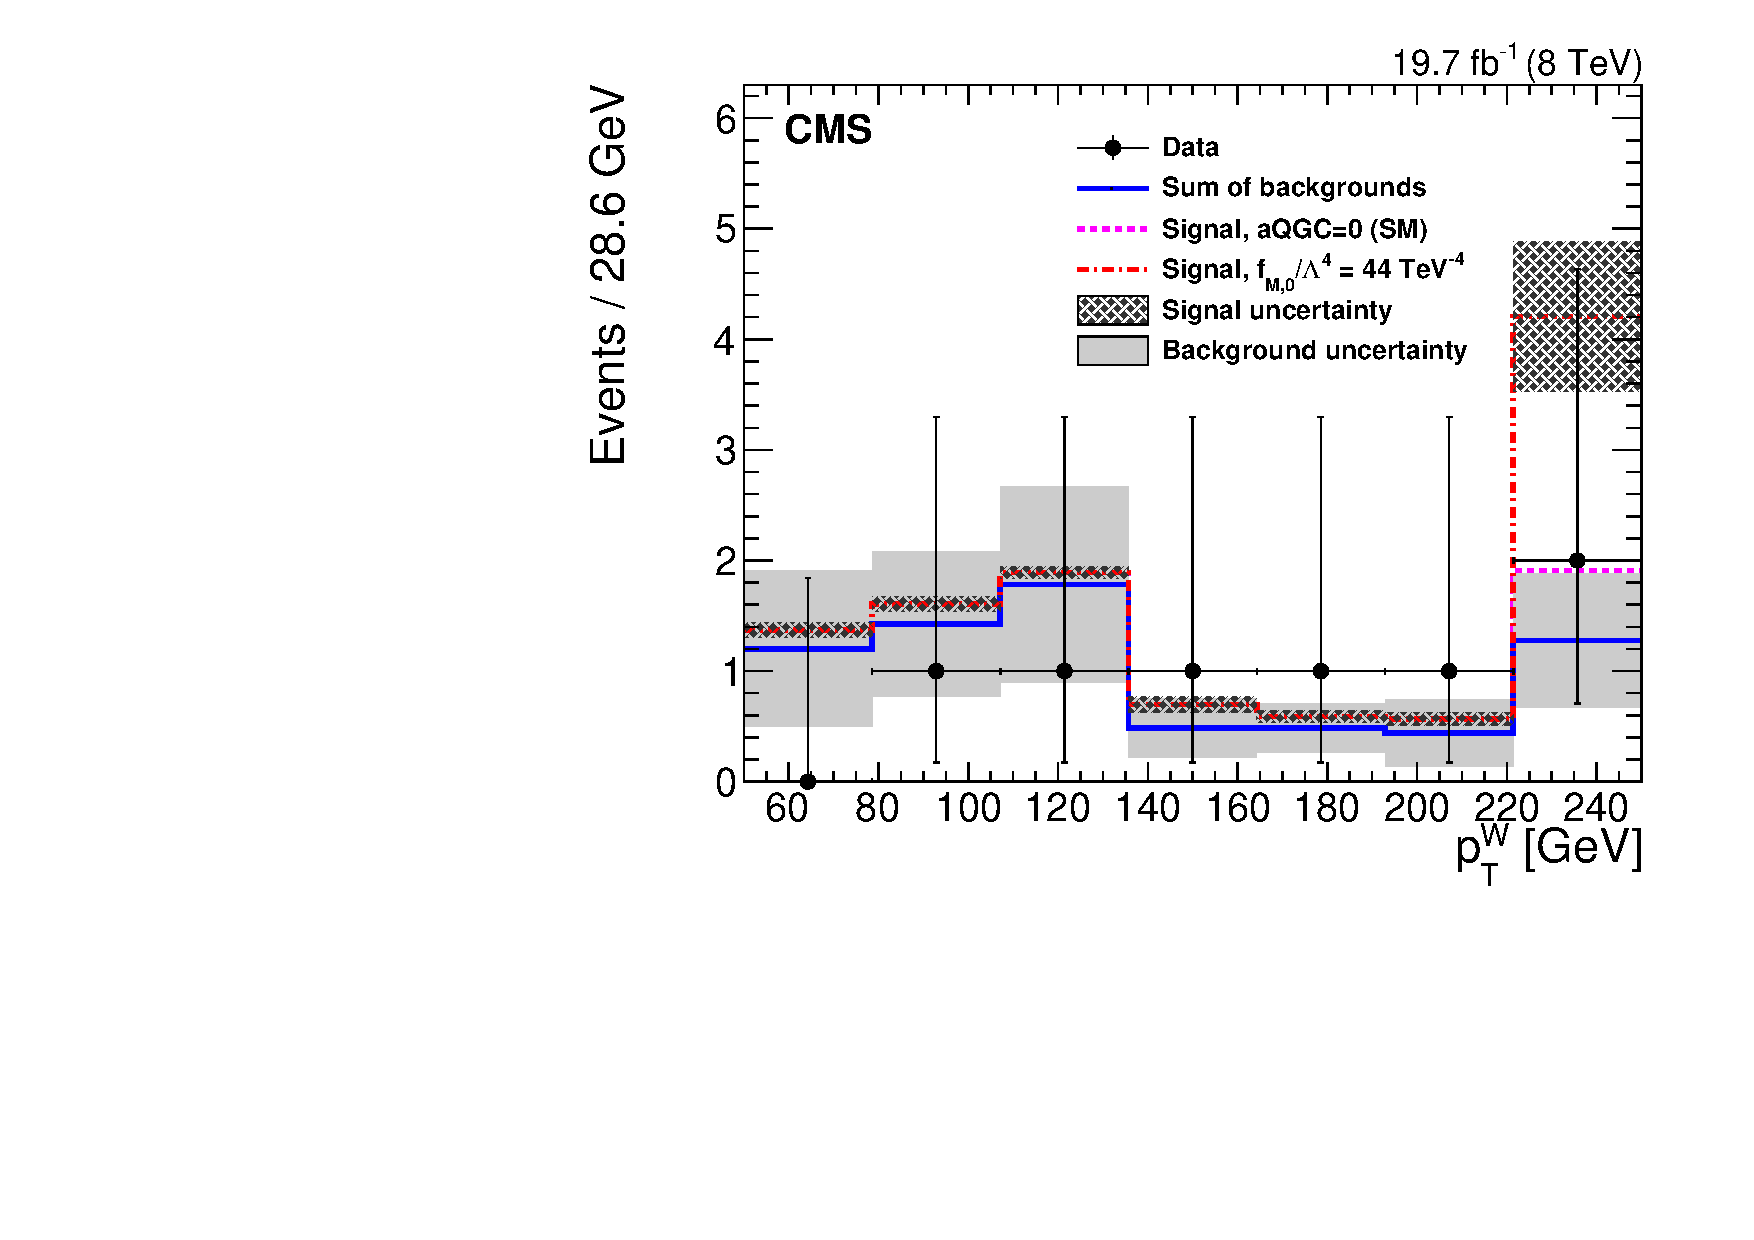
\includegraphics[width=3in]{Figure-9.pdf}
% TODO: 中英还是不匹配?(221.4 什么的)
\cnenfigcaption{合并电子与 $\mu$ 子道的 W 玻色子的横动量分布. 最后一段包括所有 $\text{p}^{\Wboson}_{\text{T}} > 221.4$ GeV 的事例. 其中粉色虚线为标准模型的信号贡献, 红色虚线为反常耦合算符取 $f_{M,0}/\Lambda^4 = 44$ TeV\textsuperscript{−4} 时的信号贡献. 图中灰色部分代表统计和系统误差之和}{Comparison of predicted and observed $\text{p}^{\Wboson}_{\text{T}}$ distributions with the combined electron and muon channels. The last $\text{p}^{\Wboson}_{\text{T}}$ bin has been extended to include the overflow contribution. The dash-dotted line depicts a representative signal distribution with anomalous coupling parameter $f_{M,0}/\Lambda^4 = 44$ TeV\textsuperscript{−4} and the dashed line shows the same distribution corresponding to the SM case. The bands represent the statistical and systematic uncertainties in signal and background predictions summed in quadrature}
\label{fig:9}
\end{figure}

\subsection{$\Zboson\gamma$散射}

$\Zboson\gamma$道\upcite{26}和$\Wboson\gamma$道类似, 由于光子的存在, $\Zboson\gamma$道不与电弱对称自发破缺直接联系, 其主要的物理意义在于对反常耦合的研究. 与$\Wboson\gamma$不同的是, Z玻色子和光子都是中性粒子, 因此这个道对四个中性玻色子耦合顶点敏感, 例如Zggg顶点. $\Zboson\gamma$的道主要本底为QCD本底和非瞬发光子本底. 其中非瞬发光子本底来自于Z玻色子+喷注过程, 和$\Wboson\gamma$道类似, 绝大部分的非瞬发光子来自于$\pi^0$介子的衰变, 因此这部分本底的估计和$\Wboson\gamma$道是一样的. 另外一个主要本底是具有QCD顶点的$\Zboson\gamma$过程, 这部分本底的估计由蒙特卡洛样本估计. 通过要求150 GeV $< \mass_{\text{jj}} < $ 400 GeV可以定义一个控制区域, 在这个区域内信号过程贡献很小, 将这部分的QCD本底做缩放, 使得控制区域的所有本底与数据符合, 将缩放系数应用到QCD本底上. QCD本底的缩放系数为$1.00\pm0.22$, 这个值与文献中在 $\mass_{\text{jj}} <$ 400 GeV区域的NLO/LO的$K$系数1.1大致接近. 其他的本底, 通过一系列的动力学变量选择, 总的贡献小于总本底事例数的10\%. 

$\Zboson\gamma$道利用的是Z玻色子和光子的不变质量来研究反常耦合. 图 \ref{fig:10} 中显示了一个反常耦合算符取特定值时的事例与数据的分布图, 数据与标准模型预测在误差内符合. 

\section{二期数据的VBS分析}

CMS合作组利用一期取数进行了许多Higgs玻色子相关的分析, 除此之外, 还进行了许多新物理的寻找. 不过大量关于新物理的分析并没有得到期望的结果, 因此标准模型相关的分析也再次成为人们重点关注的方向. 除了第 \ref{sec:3} 节中提到的三个工作, CMS利用二期数据还进行了WZ和ZZ道的测量. 以下将对利用二期数据的工作进行介绍. 

\begin{figure}[ht!]
\centering
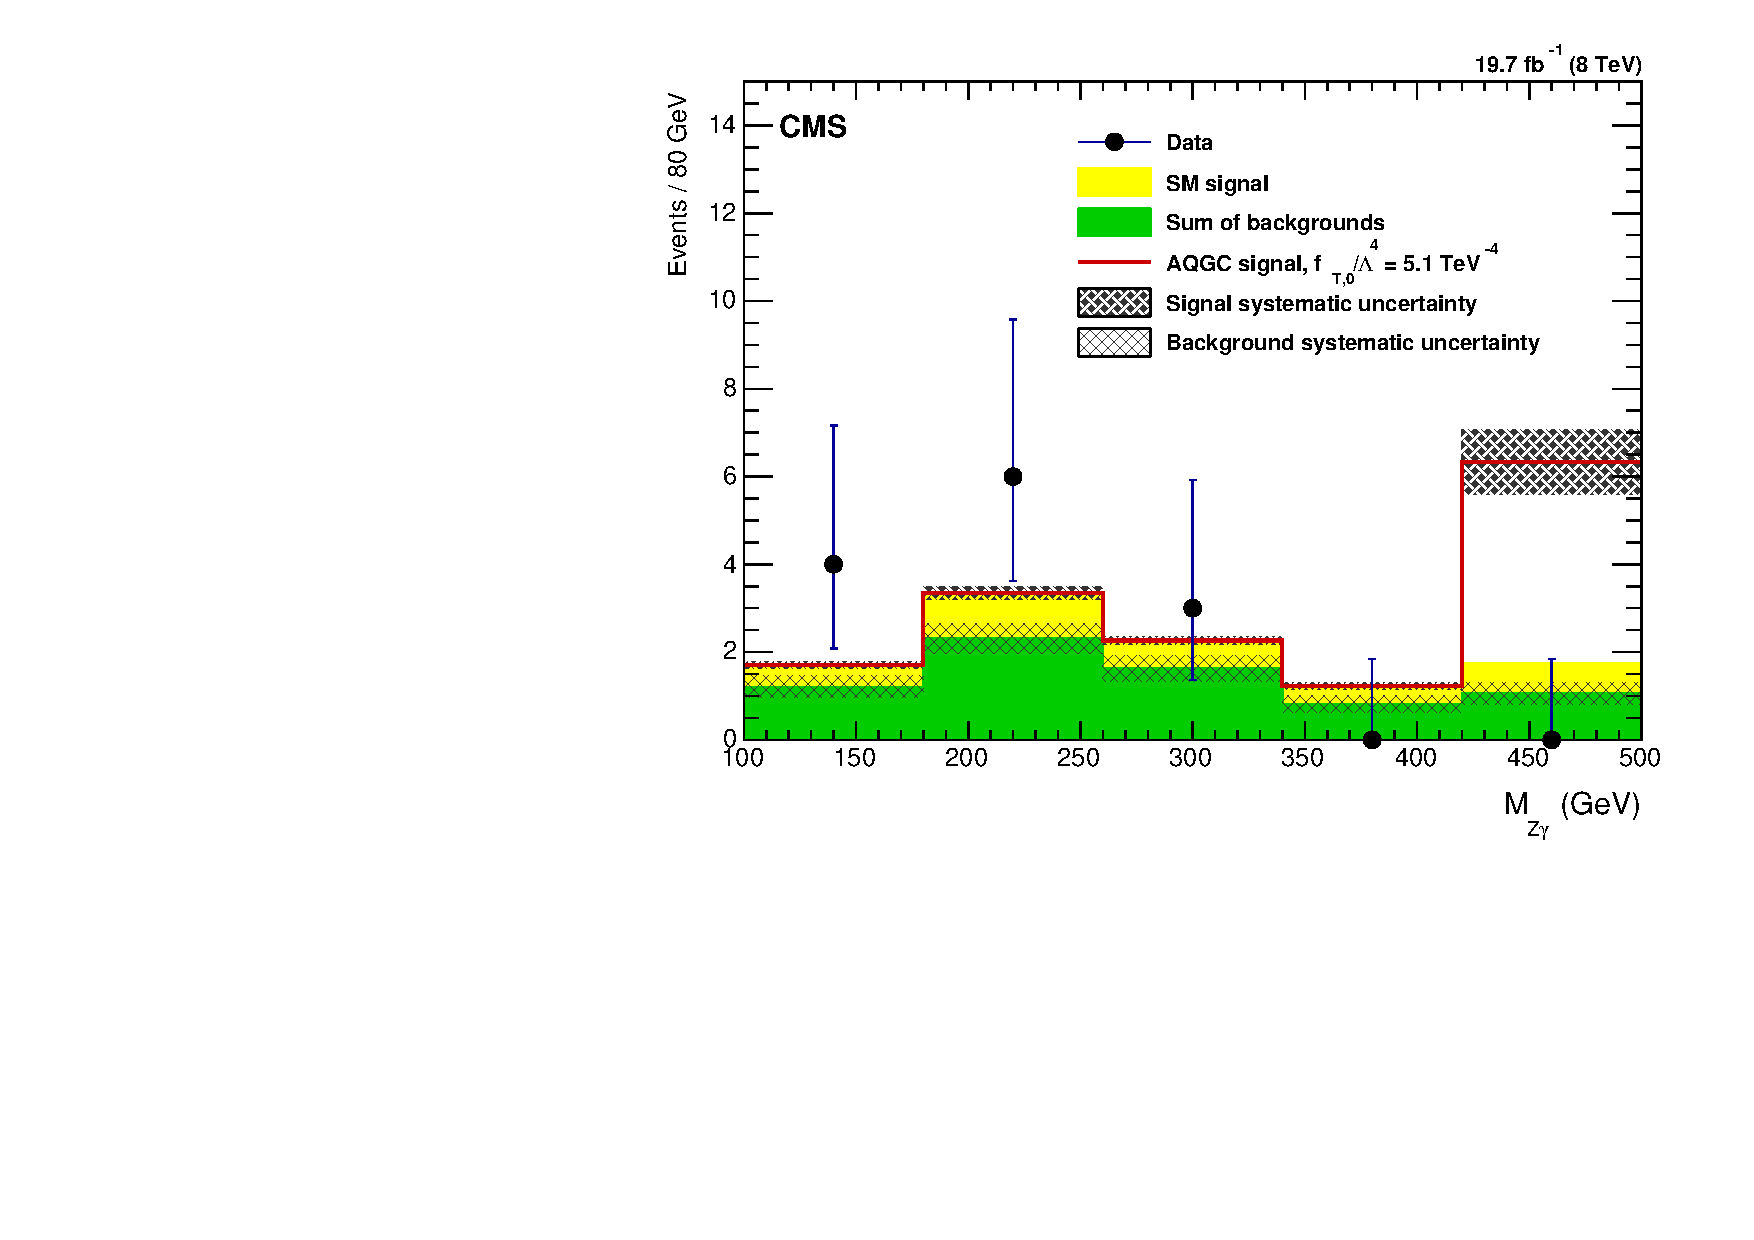
\includegraphics[width=3in]{Figure-10.pdf}
\cnenfigcaption{Z 玻色子和光子不变质量分布. 最后一段包括所有 $\mass_{\Zboson\gamma} > 420$ GeV 的事例. 其中红线为反常耦合算符取特定值时的信号贡献, 阴影部分表示样本的统计误差和系统误差之和. 黑点及误差棒表示测量事例数及其统计误差}{The invariant mass distribution of the $\Zboson\gamma$ system. The highest mass bin includes events with $\mass_{\Zboson\gamma} > 420$ GeV. Error bars represent the statistical uncertainty in the data, while the systematic uncertainties in the aQGC signal and background estimate are shown as hatched bands}
\label{fig:10}
\end{figure}

\subsection{同号WW散射}
利用二期数据的分析的物理目标和一期基本是一致的, 但是2016年数据对应的积分亮度为36 fb\textsuperscript{-1}, 更精细的测量则需要更多的数据. 同号WW散射\upcite{27}的本底分析和一期的分析大致类似, 最重要的两项本底为非瞬发轻子和WZ的贡献. 

二期数据的对撞质心系能量为13 TeV, 而且有更高的积分亮度. 两个轻子的动量选择条件比一期的更严, 来适当地减少我们不感兴趣的信号事例及本底. 对于包含顶夸克的本底, 利用底夸克标记技术来排除\upcite{42,43}. 对于非瞬发轻子, 要求两个轻子的不变质量大于20 GeV来压低贡献. 对于WZ本底, 同样要求事例只有两个轻子来排除之. 

与一期分析不同的是, 二期分析利用两个轻子的不变质量以及两个喷注的不变质量来抽取信号过程的显著度. 电弱过程的同号WW散射对应的测量(预期)显著度为5.5(5.7)倍标准偏差. 这是LHC上第一个以超过5倍标准偏差发现的VBS过程, 这个结果对于电弱对称自发性破缺的研究具有重要意义, 同时也为之后的纵向极化的同号WW散射过程提供了基础. 与一期类似, 这个工作也给出了几项反常耦合算符的上限, 以及不同质量的双电荷Higgs玻色子衰变的截面上限. 

\subsection{$\Wboson\gamma$散射}
同样地, 利用2016年数据的$\Wboson\gamma$\upcite{28}的工作的物理目标和一期分析类似, 一是测量该VBS过程, 二是研究反常耦合. 

\ref{sec:3.2} 小节中提到的本底分析也被应用到二期工作中. 值得注意的是, 二期分析还额外考虑了两项本底, 非瞬发轻子本底, 以及轻子和光子都是非瞬发的情况. 由于一期数据对应的对撞质心系能量更低以及积分亮度更小, 因此这两项本底的贡献不是非常明显, 而且也在一定程度上被较大的系统误差覆盖. 但是在2016年的工作中, 在$\mu$子道, 非瞬发轻子本底占总本的10\%左右, 在电子道更是达到了20\%. 另外一项的额外本底的贡献不大. 一期的工作只考虑桶部探测器部分的光子, 二期的工作还考虑了端部探测器部分的光子. 

$\Wboson\gamma$道利用喷注不变质量、以及轻子和光子的不变质量来抽取信号显著度. 通过喷注的不变质量, 将相空间分为控制区域(200 GeV $< \mass_{\text{jj}} <$ 400 GeV)和信号区域(500 GeV $< \mass_{\text{jj}}$). 图 \ref{fig:11} 为电子+桶部光子道在信号区域的二维分布图. 结合其他三个道, 以及控制区域, 得到测量(预期)显著度为4.9(4.6)倍标准偏差. 若与一期的工作合并, 则测量(预期)显著度为5.3(4.8)倍标准偏差. 这是CMS上第二个VBS过程的发现. 

\begin{figure}[ht!]
\centering
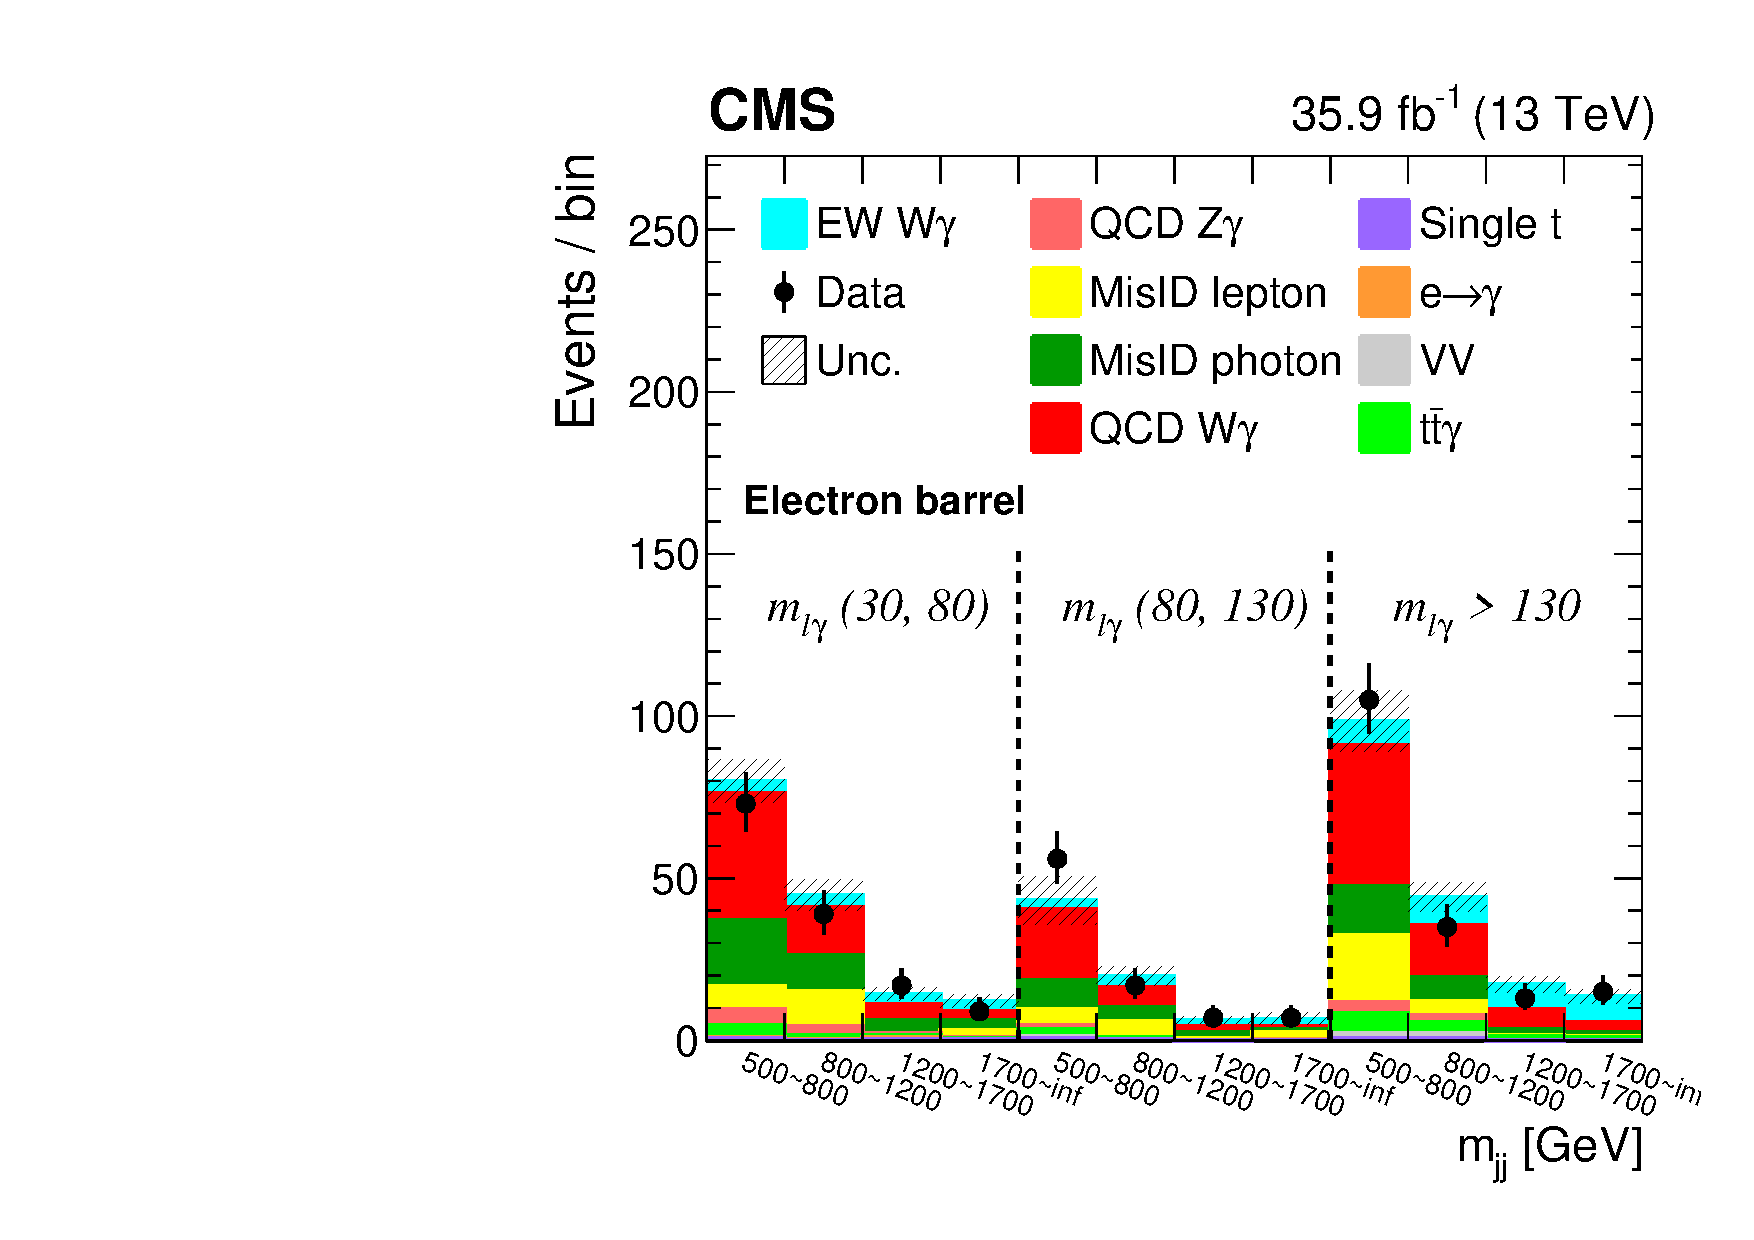
\includegraphics[width=3in]{Figure-11.pdf}
\cnenfigcaption{电子+桶部光子道在信号区域的二维分布图. 喷注不变质量分段为(0.5, 0.8, 1.2, 1.7, 无穷大) TeV, 轻子光子不变质量分段为(30, 80, 130, 无穷大) TeV. 阴影部分表示样本的统计误差和系统误差之和. 黑点及误差棒表示测量事例数及其统计误差}{The 2D distributions in signal region in the electron + barrel photon region. The $\mass_{\text{jj}}$ binning is (0.5, 0.8, 1.2, 1.7, infinite) TeV, the binning of $\mass_{l\gamma}$ is (30, 80, 130, infinite) TeV. The black points with error bars represent the data and statistical uncertainties of data, the hatched bands represent the full uncertainties of the predictions}
\label{fig:11}
\end{figure}

在研究反常耦合时, 二期的$\Wboson\gamma$道利用的变量是W玻色子和光子的不变质量. 结果显示数据与标准模型预测相符合, 因此得到了一系列的反常耦合算符的上限值. 

\subsection{$\Zboson\gamma$散射}

$\Zboson\gamma$道\upcite{44}对应的二期分析与一期分析也类似, 各项本底的估计方法沿用一期. 不同点在于二期分析将位于探测器端部的光子纳入了考虑. 与$\Wboson\gamma$道类似, $\Zboson\gamma$道也根据两个喷注的不变质量定义了控制区域和信号区域. 在抽取信号显著度时, $\Zboson\gamma$道利用的是两个喷注的不变质量和赝快度差两个变量. 图 \ref{fig:12} 为电子+桶部光子道在信号区域的二维分布图. 在结合其他三个道以及控制区域之后, 得到的测量(预期)显著度为3.9(5.2)倍标准偏差. 若与一期的工作合并, 则测量(预期)显著度为4.7(5.5)倍标准偏差. 对于反常耦合的研究发现数据和标准模型之间在误差范围内符合, 因此给出了一些反常耦合算符的上限. 

\begin{figure}[ht!]
\centering
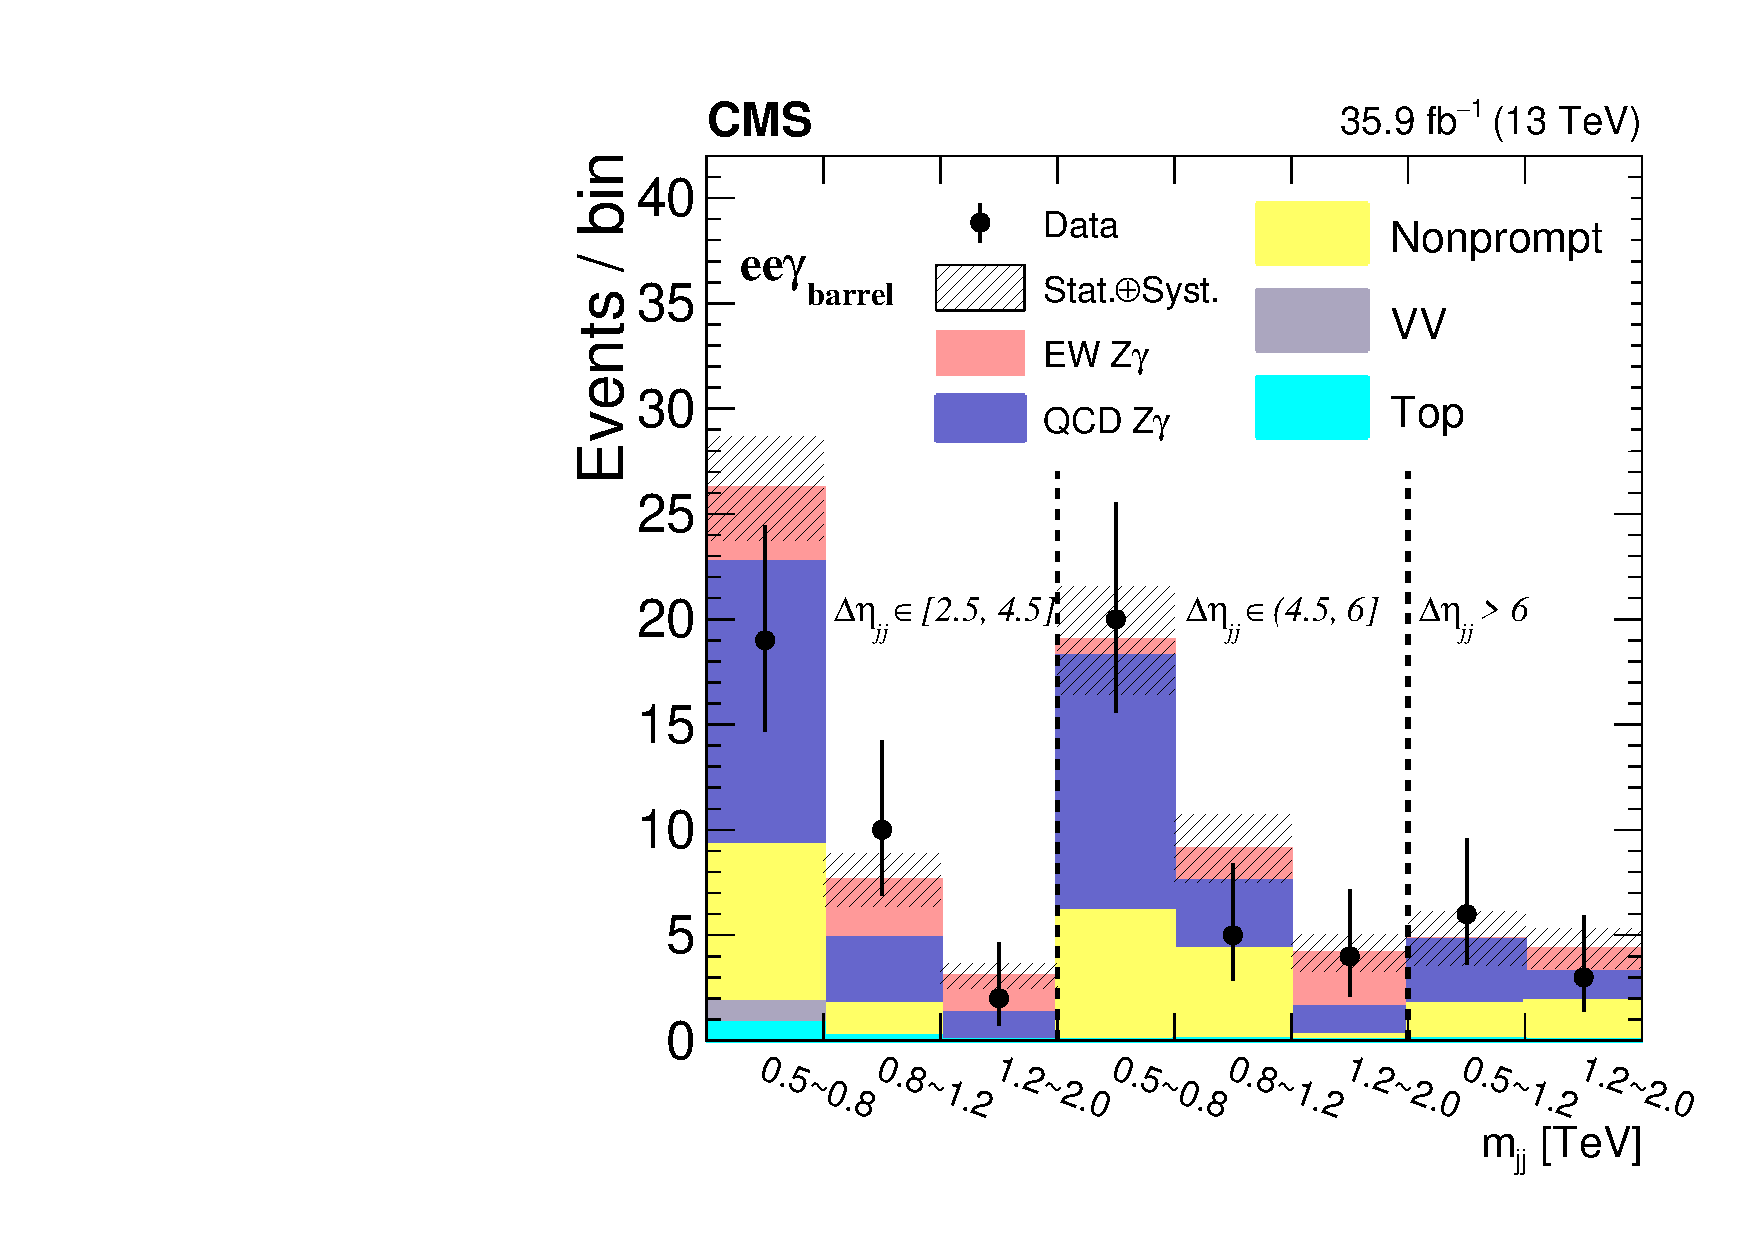
\includegraphics[width=3in]{Figure-12.pdf}
\cnenfigcaption{电子+桶部光子道在信号区域的二维分布图. 喷注不变质量分段为(0.5, 0.8, 1.2, 2.0, 无穷大) TeV, 喷注赝快度差分段为(2.5, 4.5, 6, 无穷大). 阴影部分表示样本的统计误差和系统误差之和. 黑点及误差棒表示测量事例数及其统计误差}{The 2D distributions in signal region in the electron + barrel photon region. The $\mass_{\text{jj}}$ binning is (0.5, 0.8, 1.2, 2.0, infinite) TeV, the binning of $| \Delta \eta_{\text{jj}} |$ is (2.5, 4.5, 6, infinite). The black points with error bars represent the data and statistical uncertainties of data, the hatched bands represent the full uncertainties of the predictions}
\label{fig:12}
\end{figure}

\subsection{WZ散射}

WZ道\upcite{45}的末态为两个喷注加上三个轻子, 根据轻子中电子的个数, 可以将信号分为四类. WZ道的本底分为两类, 一类为ZZ、$t$Z+喷注等, 这类本底的轻子为瞬发轻子, 例如ZZ过程衰变出4个轻子, 但是其中一个没有被探测器记录到, 而$t$Z+喷注过程则是因为顶夸克衰变得到W. 另外一类则是非瞬发轻子的贡献, 主要是Z+喷注和双顶夸克等过程, 例如Z+喷注过程中, 喷注中的强子衰变为轻子. 

瞬发轻子类的本底估计直接根据蒙特卡洛样本得到. $\Zboson\gamma$过程也属于非瞬发类轻子本底, 光子可以转化为正负轻子对, 这一过程的贡献也直接通过蒙特卡洛样本得到. 其他的非瞬发轻子本底的贡献则通过数据得到, 用到的方法和WW道、$\Wboson\gamma$道的方法类似. 

由于末态的轻子可能来自于W玻色子或者Z玻色子的衰变, 通过以下条件来构建末态的两个玻色子. 若三个轻子同味道, 则根据电荷可以将事例分为两个正电荷一个负电荷或者反之, 这三个轻子中带相反电荷的任意组合中, 不变质量最靠近Z玻色子质量的那个组合, 就视作来源于Z玻色子衰变, 余下的那个轻子则视作来自于W玻色子的衰变. 若三个轻子为不同味道, 且其中两个同味道的两个轻子带电荷相反, 则这两个轻子视作来自于Z玻色子的衰变. 为了压低来自于顶夸克本底的贡献, 要求构成Z玻色子的两个轻子的不变质量落在Z玻色子的质量窗之内. 任意两个轻子的不变质量都要大于4 GeV, 来排除理论上的红外发散以及软轻子的影响. 此外, 三个轻子的不变质量要求大于100 GeV, 来排除$\Zboson\gamma$本底. 

在抽取电弱过程的显著度时, QCD WZ过程为贡献最大的本底. WZ分析的信号区域要求了较大的喷注不变质量以及赝快度差, 通过反转这两个选择条件定义了QCD WZ过程的控制区域. QCD WZ本底的估计通过蒙特卡洛样本得到, 并且在其控制区域将QCD WZ的事例数做缩放, 使得该控制区域内的本底加上信号与数据相符, 结果显示QCD WZ的缩放系数与1吻合. 

电弱过程的信号显著度抽取利用了喷注的不变质量和赝快度差. 如图 \ref{fig:13} 所示, 信号加上本底与数据符合较好. 利用这12个bin的事例信息, 得到测量(预期)显著度为2.2(2.5)倍标准偏差. 这项工作还测量了EW+QCD WZ作为信号的截面, 测量截面时, 将信号按照电子的数目分为4个道, 联合4个道的信息做拟合, 得到了与理论相符的结果. 

\begin{figure}[ht!]
\centering
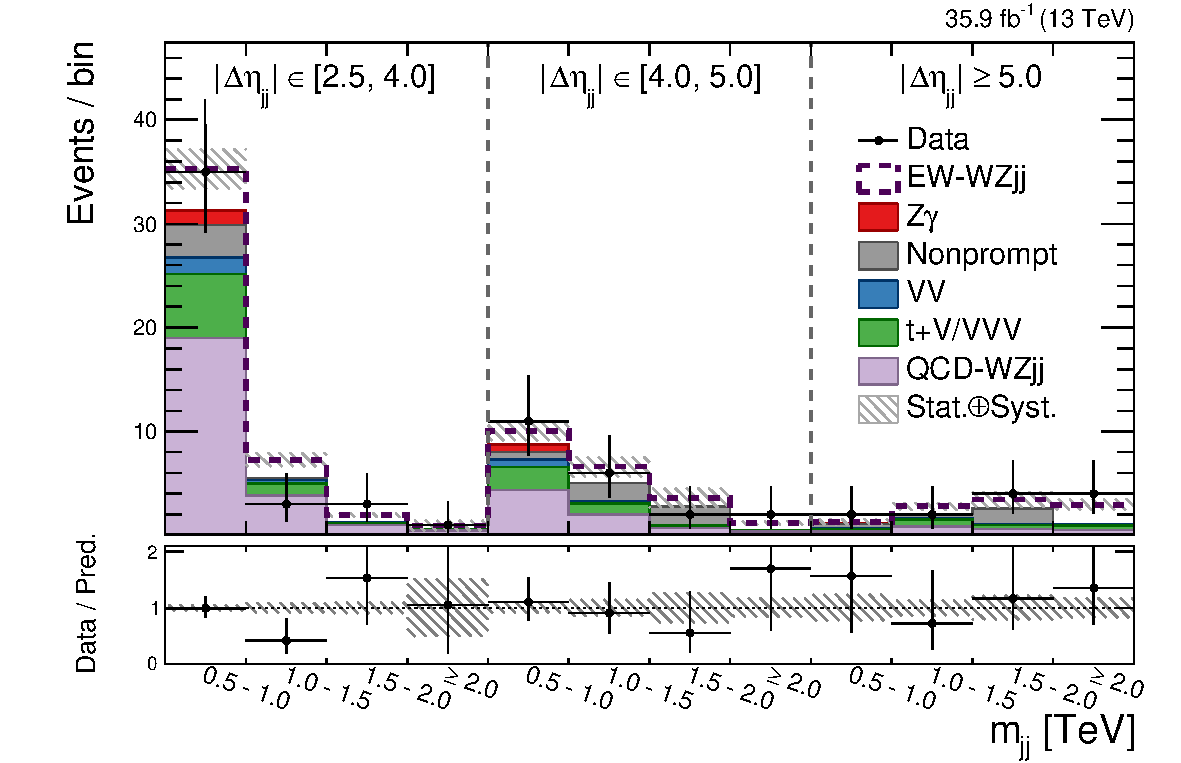
\includegraphics[width=3in]{Figure-13.pdf}
\cnenfigcaption{WZ道信号区域的二维分布图, 喷注不变质量分段为(0.5, 1.0, 1.5, 2.0, 无穷大) TeV, 赝快度差分段为(2.5, 4.0, 5.0, 无穷大). 阴影部分表示样本的统计误差和系统误差之和. 黑点及误差棒表示测量事例数及其统计误差. 底部小图表示测量事例数与预测事例数比值}{The one-dimensional representation of the 2D distribution of $\mass_{\text{jj}}$ and $|\Delta\eta_{\text{jj}}|$. The $\mass_{\text{jj}}$ binning is (0.5, 1.0, 1.5, 2.0, infinite) TeV, the binning of $| \Delta \eta_{\text{jj}} |$ is (2.5, 4.0, 5.0, infinite). The hatched bands represent the total and relative systematic uncertainties on the predicted yields. The bottom panel shows the ratio of the number of events measured in data to the total number of expected events}
\label{fig:13}
\end{figure}

WZ道除了具有通常VBS过程对反常耦合敏感的性质, 还能研究带电Higgs玻色子. 在一些对标准模型做扩展的理论中, 例如GM模型\upcite{39}中, Higgs玻色子部分包含SU(2)的三重态, 这会导致带电Higgs玻色子的存在. 这个带电玻色子与标准模型的矢量玻色子之间的耦合将会非常大, 耦合强度与带电Higgs玻色子质量以及GM模型真空期望值的混合角相关. WZ道的结果得到了一系列的反常耦合上限值, 以及不同质量下的带电Higgs玻色子衰变到WZ的分支比上限. 

\subsection{ZZ散射}

ZZ道\upcite{46}是VBS过程中非常重要的一个道, 因为两个玻色子都具有质量, 所以可以作为直接探究电弱SSB机制的探针. 另外, ZZ道是所有VBS过程中最干净的道, 其末态为4个轻子加上两个喷注, 因此可以完全重建. 虽然ZZ道有如上的优点, 但是对它的分析也存在相当大的挑战, 原因在于电弱信号过程的截面很小, 同时QCD ZZ的截面很大. 因此, 分析利用了TMVA中的提升决策树 (Boosted Decision Tree, BDT) \upcite{47}来区分信号和本底. 

正如前文所述, QCD ZZ是最重要的本底, 它又可以分为树图和圈图, 前者通过产生子$\MADGRAPH$产生, 后者为胶子与胶子之间的对撞, 通过产生子MCFM\upcite{48}产生. 其他类似于WWZ过程的包含4个瞬发轻子的本底通过$\MADGRAPH$来估计. 

由于末态具有4个轻子, 那么两个Z玻色子的重建将会有多种选择. 通过以下条件来确定两个Z玻色子的重建: 对于4个轻子, 要求能构成两对同味道不同电荷的组合, 其中不变质量更接近Z玻色子质量者重建出$\Zboson_1$, 另一个组合重建出$\Zboson_2$, 且$\Zboson_1$和$\Zboson_2$的质量都要大于40
GeV并小于120 GeV, 且要求任意的两个轻子的不变质量大于4 GeV以压低来自于强子衰变的轻子. 若有多种组合方式满足上述要求, 则选择所有组合中双轻子不变质量最接近91.2 GeV所在的那个组合. 

ZZ道总共选取了36个变量作为输入进行多变量分析, 包括两个喷注的不变质量、喷注的赝快度差以及两个Z玻色子的不变质量等. 图 \ref{fig:14} 显示了在信号区域内, 蒙特卡洛信号、本底与数据的多变量分析输出结果的分布, 从图中可以看出, 电弱信号明显地与本底区分开来, 并且信号加上本底与数据符合良好. 得到测量(预期)显著度为2.7(1.6)倍标准偏差. 除此之外, ZZ道对反常耦合的研究结果显示标准模型预期与数据符合. 

\begin{figure}[ht!]
\centering
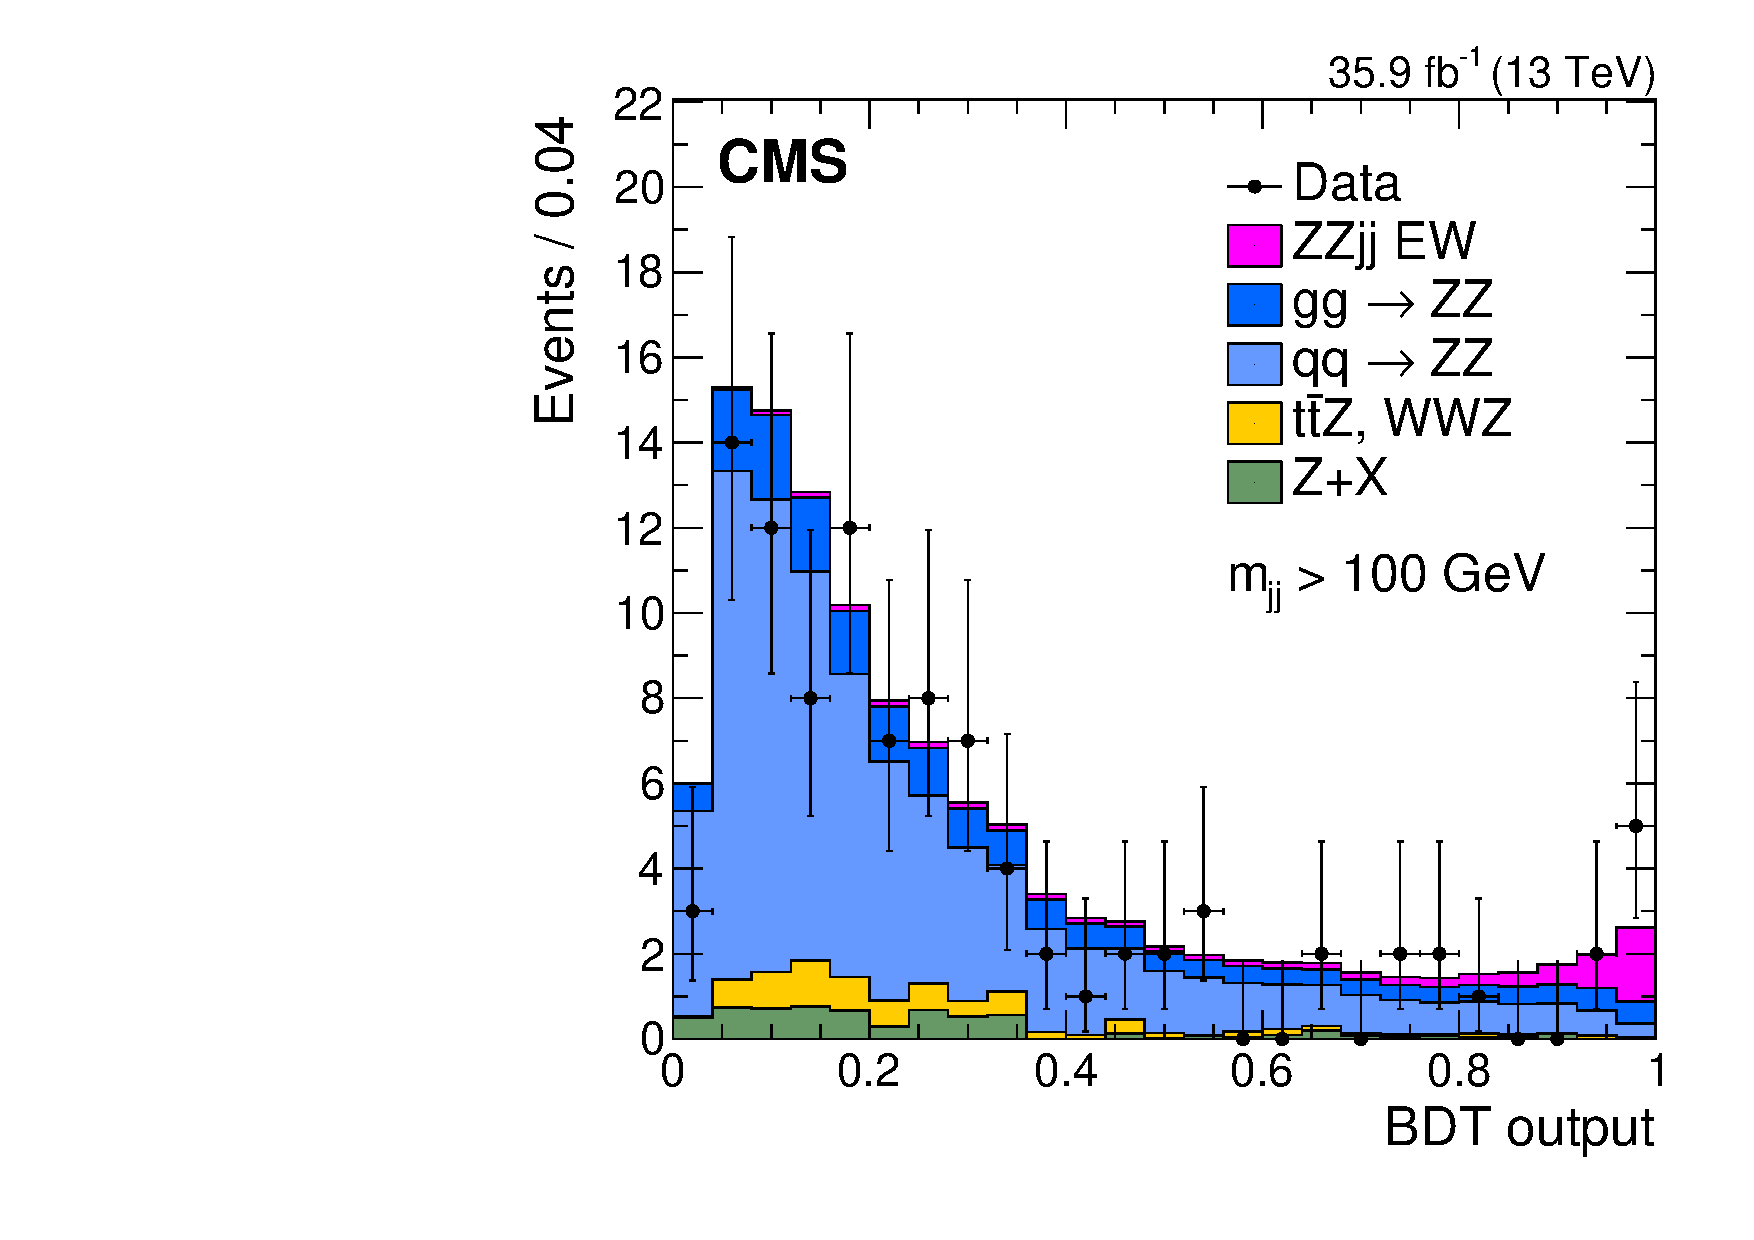
\includegraphics[width=3in]{Figure-14.pdf}
\cnenfigcaption{ZZ道信号区域内信号、本底以及数据的多变量分析输出结果分布. 柱状图为信号和本底的叠加. 黑点及误差棒表示测量事例数及其统计误差}{Distribution of the BDT output in the signal region. Points with error bar represent the data and uncertainties, filled histograms are the expected signal and background contributions}
\label{fig:14}
\end{figure}

\section{VBS过程的纵向极化测量}

随着CMS上关于VBS过程的分析日渐成熟, 对VBS过程纵向极化的测量也逐渐展开. 这些测量包括利用深度神经网络(Deep Neural Network, DNN)方法对高亮度LHC (HL-LHC)时期的预研结果, 以及近期公开的利用CMS数据对同号WW散射进行的第一次极化测量. 本节将对相关工作进行回顾. 

\subsection{DNN方法研究同号WW的纵向极化\upcite{49}}

分析样本产生流程如下: 利用产生子$\MADGRAPH$产生费曼图水平的事例$\rightarrow$ 利用产生子$\PYTHIA$模拟部分子簇射和强子化过程$\rightarrow$ 利用Delphes\upcite{50}模拟CMS探测器的响应. 

根据二期数据的同号WW分析可知, 若要求喷注不变质量大于1.5
TeV, 本底已经非常少. 也就是说, 测量纵向极化时, 两个W玻色子都是纵向偏振(\Wboson\textsubscript{L}\Wboson\textsubscript{L})作为信号过程, 一个为纵向偏振另一个为横向偏振(\Wboson\textsubscript{L}\Wboson\textsubscript{T})或者两个都为横向偏振(\Wboson\textsubscript{T}\Wboson\textsubscript{T})作为本底, 若要求很大的喷注不变质量, 那么其他本底相对于 \Wboson\textsubscript{L}\Wboson\textsubscript{T}和 \Wboson\textsubscript{T}\Wboson\textsubscript{T}来说可以忽略. 普通的DNN直接将一系列末态相关的变量作为输入, 经过训练得到区分信号和本底的DNN模型. 而工作 \cite{49} 则基于Keras库 (https://keras.io) 和TensorFlow \upcite{52}, 提出了如图 \ref{fig:15} 所示``基于粒子''的DNN模型, 即把变量按照所属物理对象打包输入, 之后再逐步地合并. 图 \ref{fig:16} 中给出了不同分析方法对应的 ROC 曲线, 即对信号和本底的区分能力. 从图中可见, ``基于粒子''的DNN模型对应的曲线下方面积 (area under curve, AUC) 最大, 区分能力最好. 

\begin{figure}[ht!]
\centering
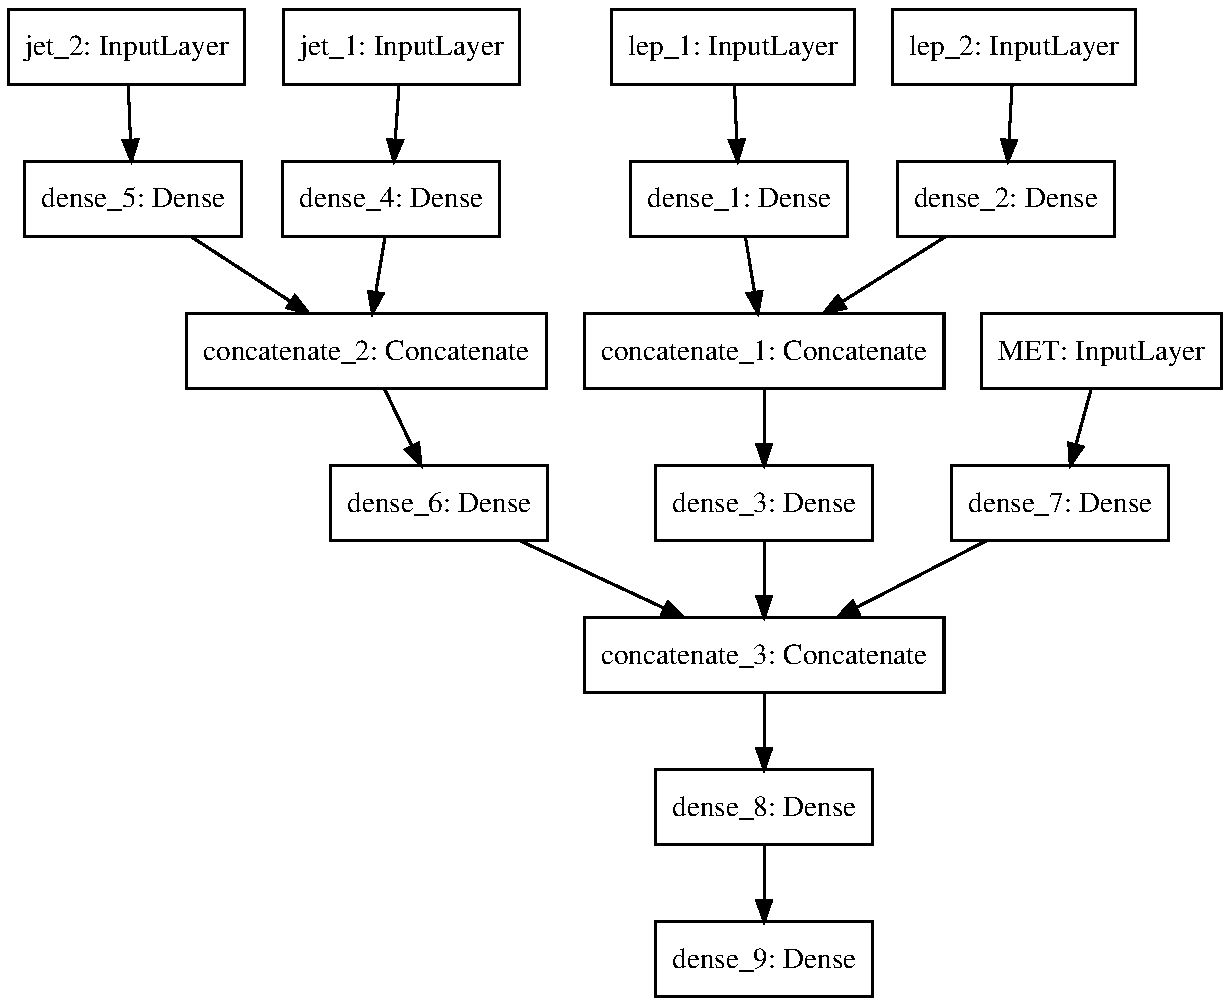
\includegraphics[width=3in]{Figure-15.pdf}
\cnenfigcaption{简化的``基于粒子''的 DNN 模型,输入变量为各种粒子的性质,且根据各个粒子打包输入}{Simplified structure of the particle-based DNN model. Inputs are features of each particle, gradually merging to the output layers}
\label{fig:15}
\end{figure}

\begin{figure}[ht!]
\centering
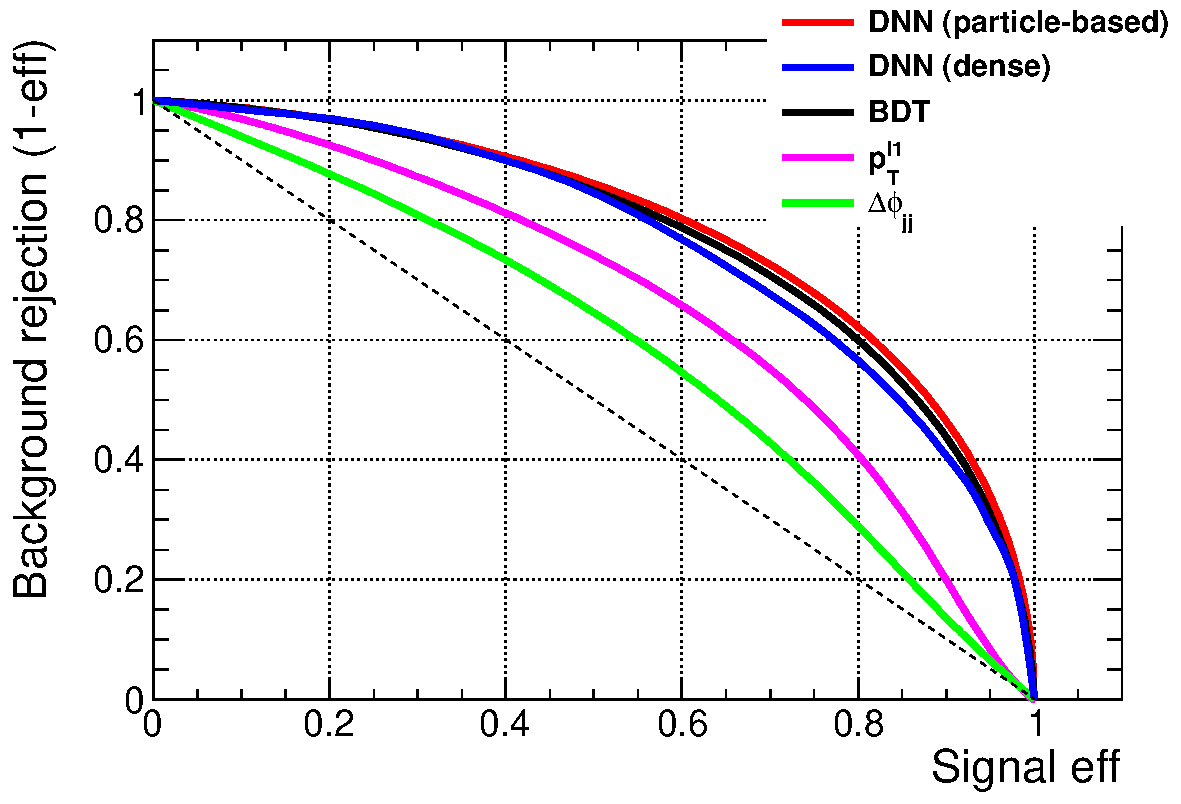
\includegraphics[width=3in]{Figure-16.pdf}
\cnenfigcaption{不同分析方法对应的ROC曲线, 横轴为纵向信号\Wboson\textsubscript{L}\Wboson\textsubscript{L}的效率, 纵轴为\Wboson\textsubscript{X}\Wboson\textsubscript{T}的排除率. 绿色曲线仅利用喷注方位角差信息, 粉色曲线仅利用领头阶轻子横动量. 黑色曲线对应BDT方法. 蓝色和红色曲线分别对应普通的DNN方法和基于粒子的DNN方法}{ROC curves of different methods. These curves stand for methods of $\Delta \phi_{\text{jj}}$, $\text{p}^{l1}_{\text{T}}$, BDT, DNN(dense) and particle-based DNN, respectively. The X-axis showing signal efficiency of LL component, and Y-axis the rejection rate of TT+TL components}
\label{fig:16}
\end{figure}

将\Wboson\textsubscript{L}\Wboson\textsubscript{L}作为信号, 且仅考虑\Wboson\textsubscript{L}\Wboson\textsubscript{T}和\Wboson\textsubscript{T}\Wboson\textsubscript{T}作为本底时, 对本底施加一定的误差, 得到了在不同选择条件下信号过程的显著度, 如图 \ref{fig:17} 所示. 从图中可以看出该模型相对于另外两种方法有很大的提升, 当喷注不变质量大于2
TeV时, 利用CMS在HL-LHC的积累的数据, 结合``基于粒子''的DNN模型, 纵向极化信号的显著度为4倍标准偏差. 若结合ATLAS的数据, 信号显著度可以超过5倍标准偏差. 

\begin{figure}[ht!]
\centering
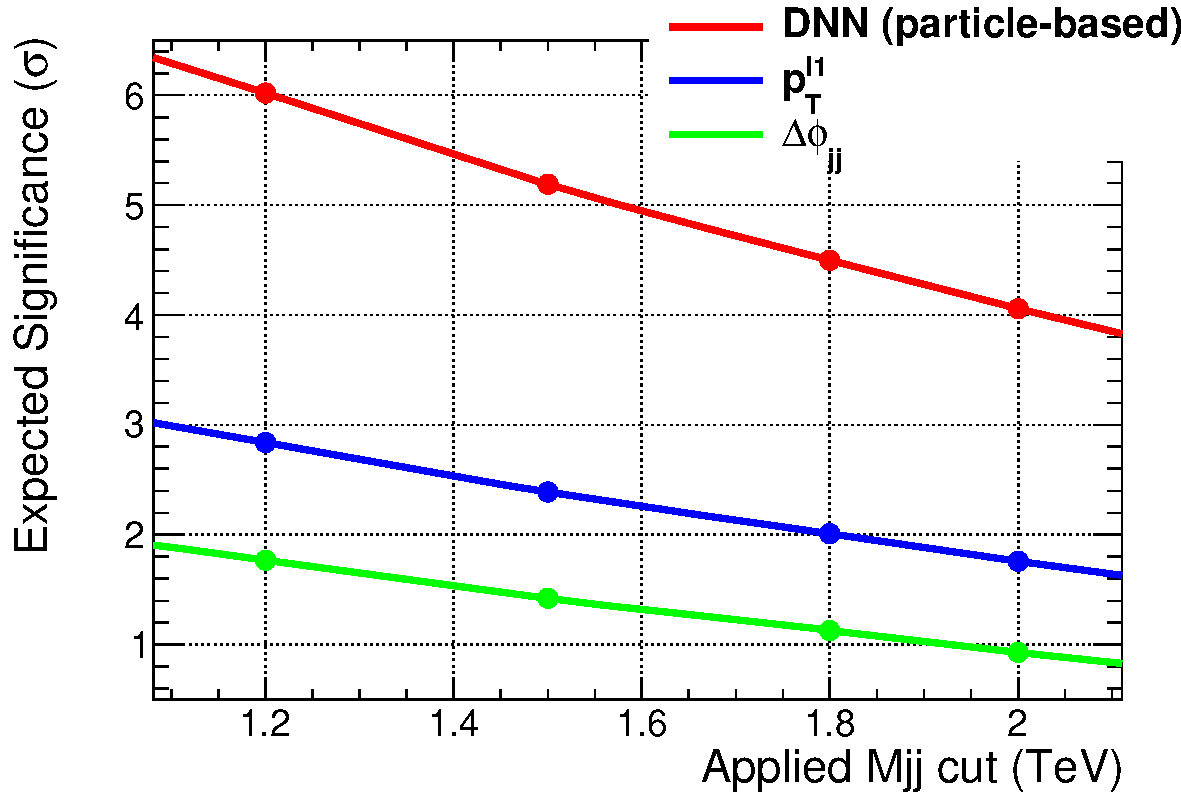
\includegraphics[width=3in]{Figure-17.pdf}
\cnenfigcaption{三种方法在不同选择条件下对应的信号显著度. 对比 $\text{p}^{l1}_{\text{T}}$ 和 $\Delta\phi_{\text{jj}}$ 方法, DNN 方法极大改进了性能}{Significance dependence on $\mass_{\text{jj}}$ selection, through fitting $\text{p}^{l1}_{\text{T}}$, $\Delta\phi_{\text{jj}}$, or the DNN discriminant. Greatly improved performance is found with DNN}
\label{fig:17}
\end{figure}

\subsection{DNN方法研究ZZ散射的纵向极化\upcite{53}}

在5.1工作的基础上, 类似的方法被应用到了ZZ散射上. ZZ散射的样本产生流程和同号WW类似. 不同于WW的地方在于ZZ散射需要考虑更多的本底. 即使设定很严格的选择条件, 除了其他偏振模式外, QCD
ZZ的贡献也是不能忽略的. 

ZZ散射的DNN模型和WW的类似, 不同点在于前者的模型将DNN方法与主成分分析(Principle Component Analysis, PCA)\upcite{54}方法相结合, 得到了区分信号与本底能力更强的模型. 图 \ref{fig:18} 表示的是信号和两种本底的PC1 (第一主要分量)和PC2 (第二主要分量)的二维分布. 

如图 \ref{fig:19} 所示, 图中表示了5种方法对应的ZZ散射中纵向极化分量的信号显著度, 红色标记表示对信号和本底施加了统计误差以及10\%的系统误差. 从图中可以看到, 利用深度神经网络方法结合PC123, CMS在HL-LHC收集的数据对ZZ散射的预期信号显著度为1.65倍标准偏差. 

\begin{figure}[ht!]
\centering
\begin{minipage}[c]{0.48\textwidth}
\centering
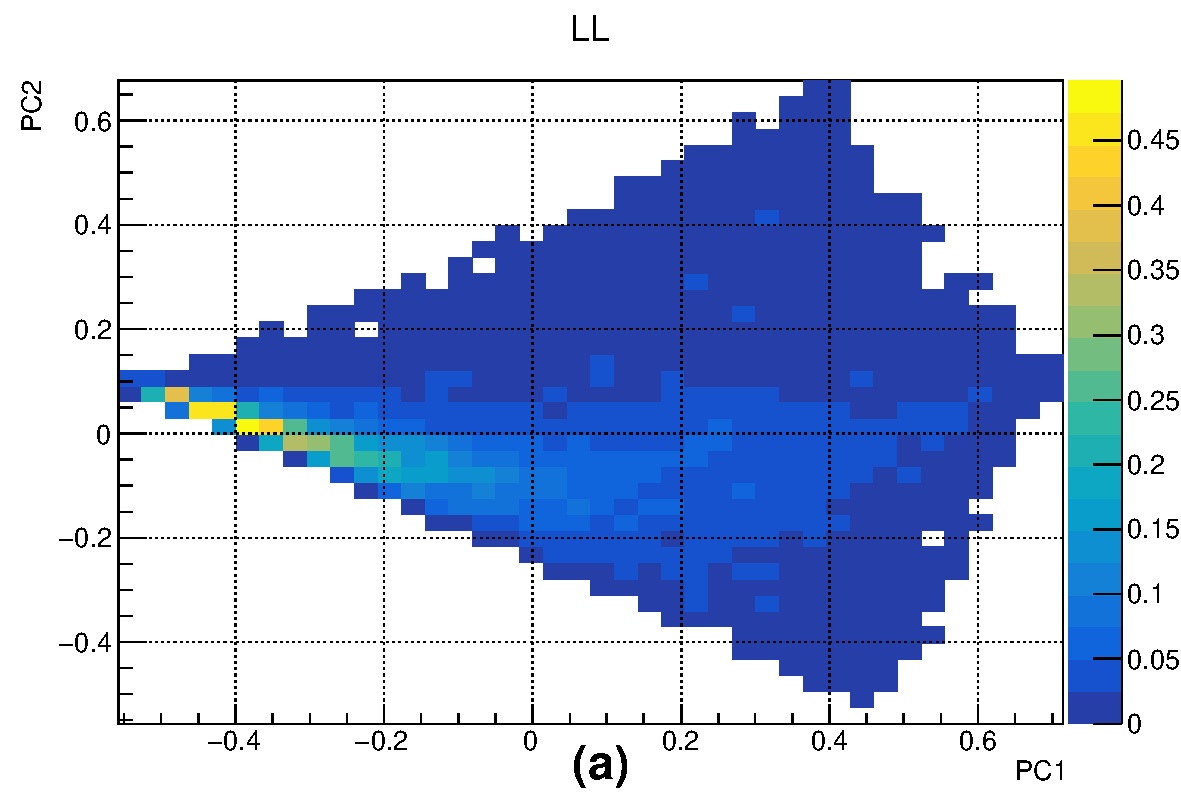
\includegraphics[width=2.5in]{Figure-18a.pdf}
\end{minipage}
\hspace{0.02\textwidth}
\begin{minipage}[c]{0.48\textwidth}
\centering
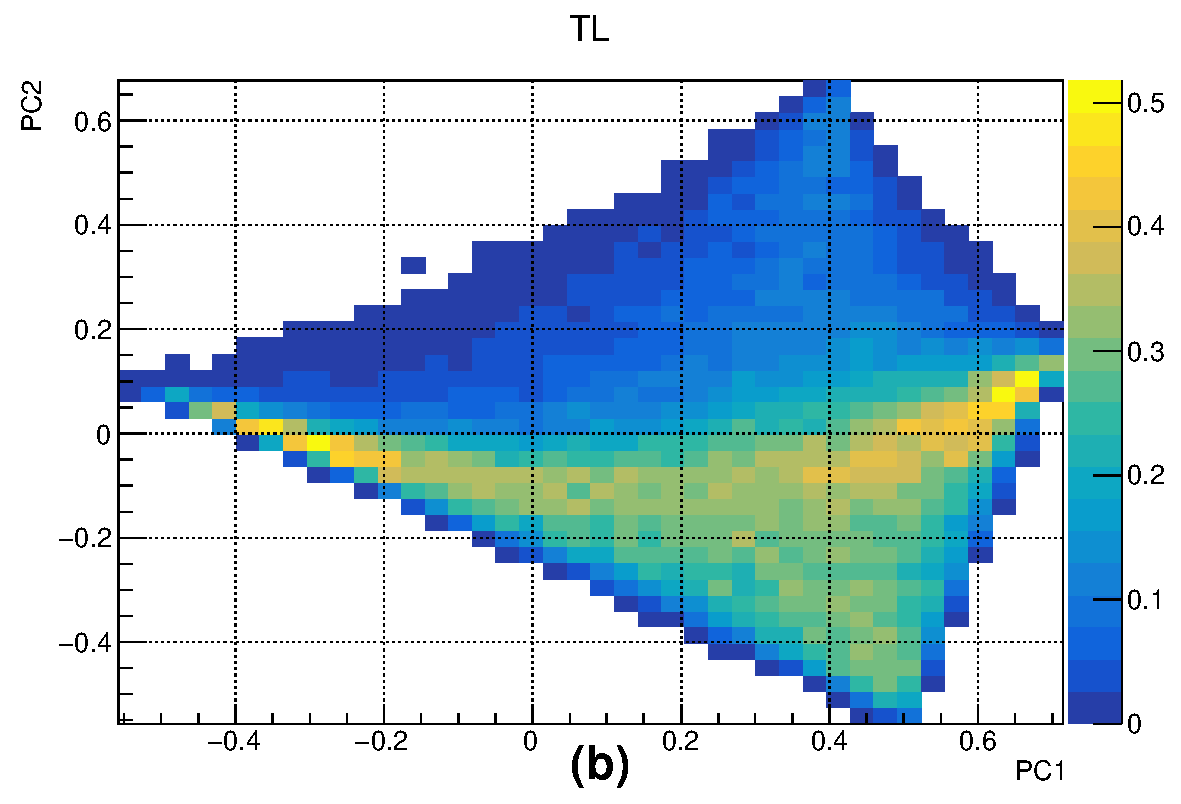
\includegraphics[width=2.5in]{Figure-18b.pdf}
\end{minipage}\\[3mm]
\hspace{0.02\textwidth}
\begin{minipage}[c]{0.48\textwidth}
\centering
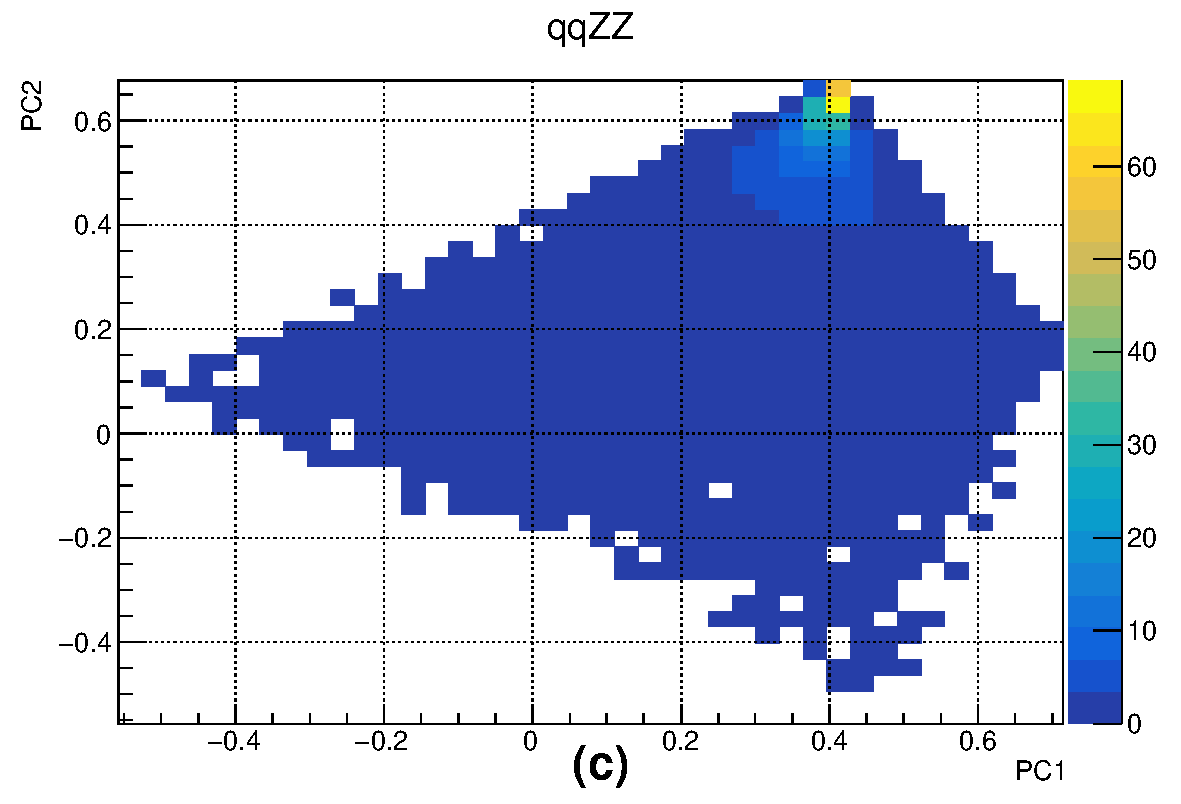
\includegraphics[width=2.5in]{Figure-18c.pdf}
\end{minipage}
\cnenfigcaption{信号(a)与其他两项本底(b)、(c)的PC1和PC2的二维分布图. 每个图都归一到相应的预期事例数}{Two dimensional histograms based on PC1 and PC2. (a), (b), and (c) correspond to the LL, TL and qqZZ samples, respectively. Each histogram is normalized to the expected yield}
\label{fig:18}
\end{figure}

\begin{figure}[ht!]
\centering
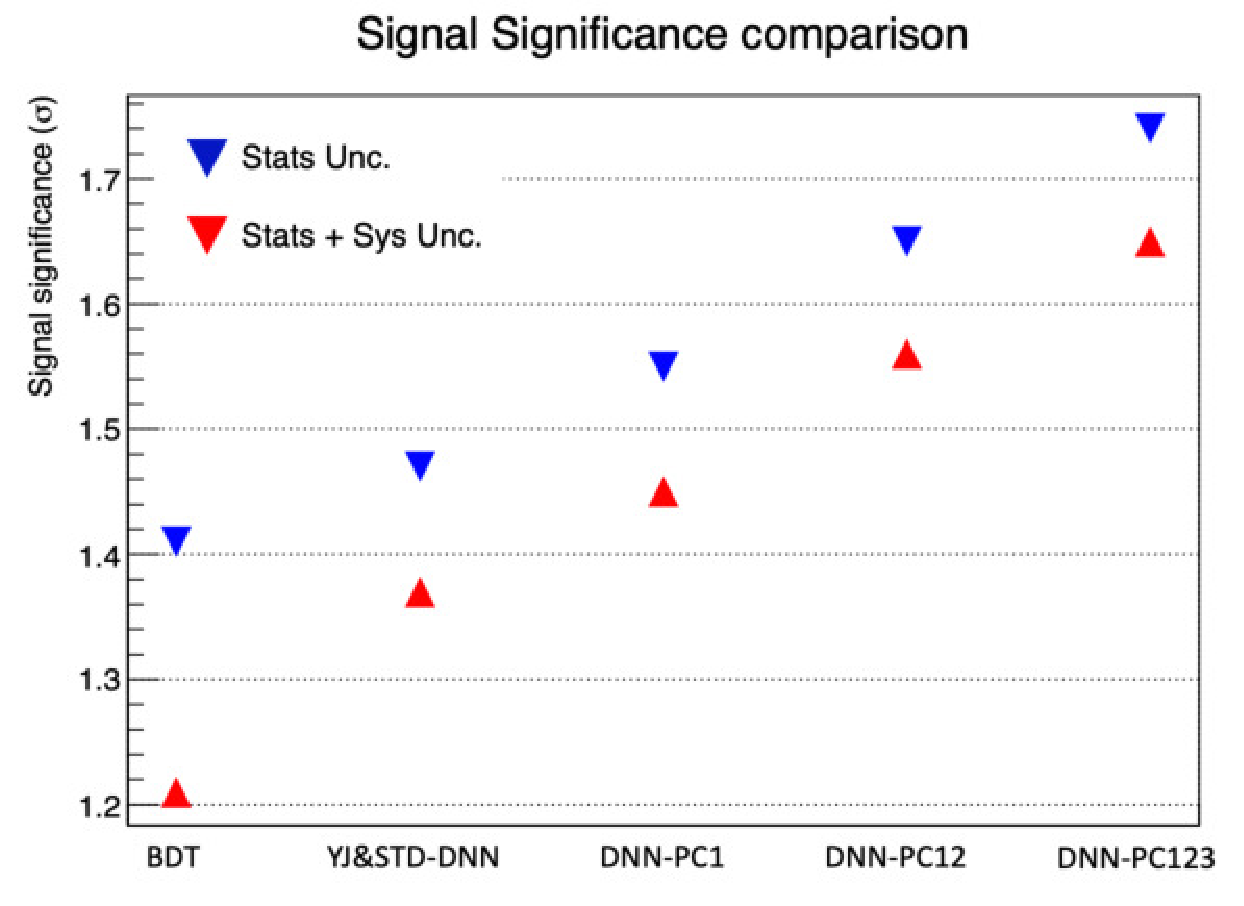
\includegraphics[width=3in,height=2.25in]{Figure-19.pdf}
\cnenfigcaption{不同方法得到的纵向极化分量的信号显著度, 蓝色标记为只考虑统计误差, 红色标记为考虑统计误差以及10\%的系统误差}{Expected signal significances obtained with the various algorithms. The blue triangles were calculated with only statistical uncertainties, while the red triangles were calculated with both statistical and systematic uncertainties}
\label{fig:19}
\end{figure}

\subsection{CMS对同号WW散射的极化测量\upcite{55}}

CMS在2016至2018年收集的数据对应的积分亮度为137 fb\upcite{56,57,58}, 大量的数据使得对VBS过程的极化测量真正成为可能. 

这项工作的关键部分为极化样本的产生, 最新版本的$\MADGRAPH$\upcite{59}产生子可以分别产生不同极化的WW过程. 工作 \cite{55} 通过对比$\MADGRAPH$和PHANTOM产生的样本, 确认了二者的一致性. 对于同号WW散射过程, 次级阶(QCD和电弱)对领头阶的修正将达到10\%$\sim$15\% \upcite{60,61}, 这样大的修正显然是不能直接忽略的. 但是由于没有对极化部分的次级阶修正, 因此直接将由非极化样本得到的修正因子应用到极化样本上. 对于 \Wboson\textsubscript{T}\Wboson\textsubscript{T}部分的修正同时考虑了QCD和电弱的修正, 而对于其他两种极化部分则只考虑了QCD的次级阶修正. 不同极化分量之间的干涉效应相对于这些分量本身是比较小的\upcite{59}, 因此不考虑干涉项的贡献. 

其他本底的产生与估计和同号WW散射类似. 对于VBS过程来说, 两个喷注的特性, 即不变质量及赝快度差, 是它与其他本底过程的重要差异. 但是对于VBS的不同极化分量, 喷注的性质基本是一样的, 主要的差异来源于W玻色子衰变的轻子相对于W玻色子的出射角分布. 另外, 纵向极化的W玻色子从入射部分子出射的角度相对于横向极化的W玻色子更小, 这就导致了横向极化的W玻色子将会倾向于携带更大的横动量. 在测量极化信号时, 最好的结果是能分别测量出三种极化分量, 但是由于统计量的限制, 只能对 \Wboson\textsubscript{T}\Wboson\textsubscript{X}和 \Wboson\textsubscript{L}\Wboson\textsubscript{X}进行测量, 其中X代表L或者T, 也就是说对应着两种信号抽取. 

为了能区分VBS的不同极化分量以及其他本底, 这项工作采用多变量分析方法来得到区分信号和本底的模型. 除了BDT之外, 文章也利用深度神经网络方法来区分信号和本底, 得到了和BDT分析类似的结果. 图 \ref{fig:20} 为测量 \Wboson\textsubscript{L}\Wboson\textsubscript{L}和 \Wboson\textsubscript{T}\Wboson\textsubscript{X}时信号和本底对应的BDT输出分布. 同样地, 测量 \Wboson\textsubscript{T}\Wboson\textsubscript{T}和 \Wboson\textsubscript{L}\Wboson\textsubscript{X}时也有对应的分布. 除了对不同极化分量进行多变量分析, 将总的同号WW过程作为信号, 也有对应的BDT输出分布. 在进行信号抽取时, 结合极化分量的BDT部分以及总的同号WW过程的BDT分布, 加上各个控制区域内的$\mass_{\text{jj}}$分布, 进行信号区域和控制区域的联合拟合. 在WW的静止系内, \Wboson\textsubscript{L}\Wboson\textsubscript{X}的测量(预期)信号显著度为2.3(3.1)倍标准偏差, 在入射质子-质子静止系内, 测量(预期)信号显著度为2.6(2.9)倍标准偏差. 由于极化态的定义与坐标系的选取有关, 因此这两种结果是和预期相符合的. 

\begin{figure}[ht!]
\centering
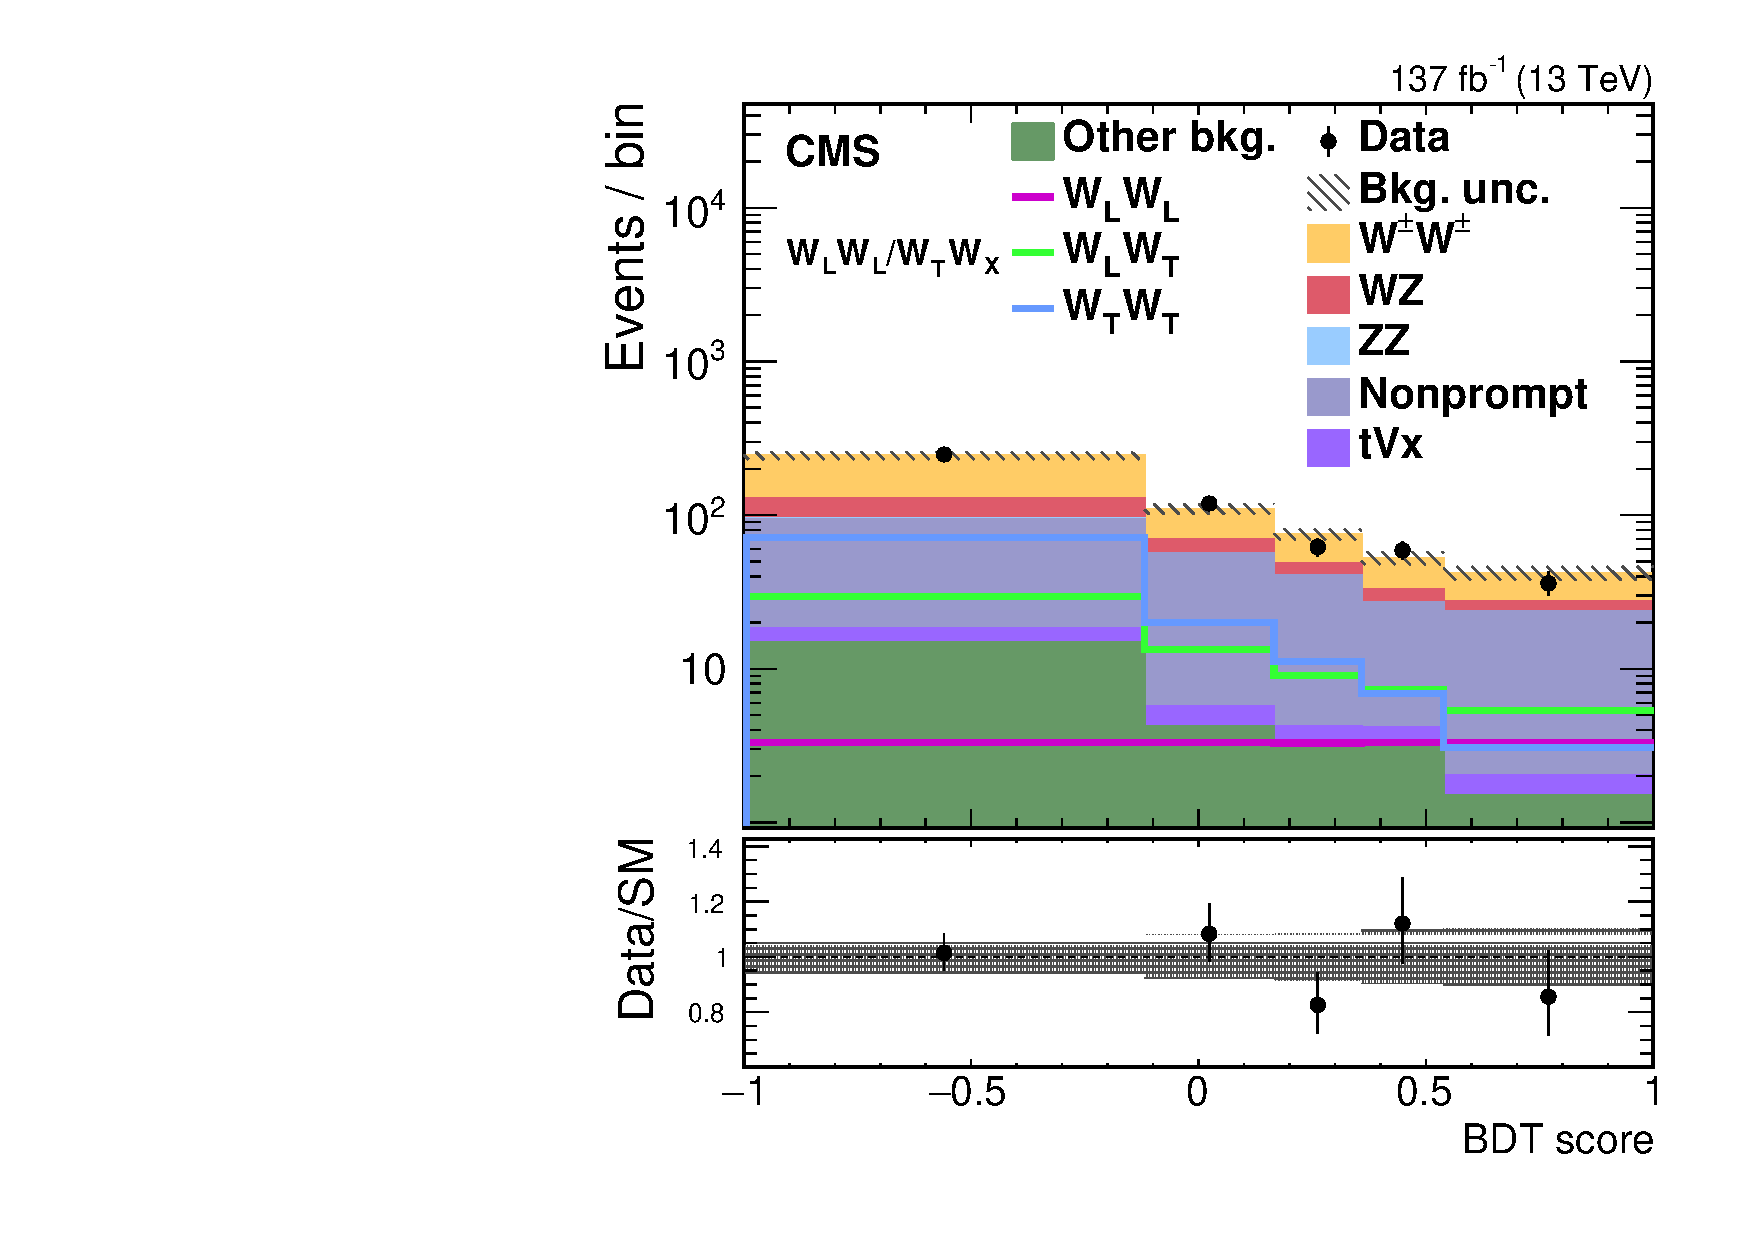
\includegraphics[width=3in]{Figure-20.pdf}
\cnenfigcaption{测量$\Wboson$\textsubscript{L}$\Wboson$\textsubscript{L}和$\Wboson$\textsubscript{T}$\Wboson$\textsubscript{X}时信号和本底对应的BDT输出的分布, 其中``$\Wboson^{\pm}\Wboson^{\pm}$''包括了电弱的极化部分(图中实线)、QCD $\Wboson^{\pm}\Wboson^{\pm}$ 以及它们的干涉项. 黑点及误差棒为测量的事例数及误差. 下部分小图代表测量事例数与预测事例数的比值, 灰色阴影部分为预测事例数的总误差}{Distributions of the output score of the signal BDT used for the $\Wboson^{\pm}$\textsubscript{L}$\Wboson^{\pm}$\textsubscript{L} and $\Wboson^{\pm}$\textsubscript{X}$\Wboson^{\pm}$\textsubscript{T} cross section measurements.  The histograms for $\Wboson^{\pm}\Wboson^{\pm}$ process include the
contributions from the $\Wboson^{\pm}$\textsubscript{L}$\Wboson^{\pm}$\textsubscript{L}, $\Wboson^{\pm}$\textsubscript{L}$\Wboson^{\pm}$\textsubscript{T}, and $\Wboson^{\pm}$\textsubscript{T}$\Wboson^{\pm}$\textsubscript{T} processes (shown as solid lines), QCD $\Wboson^{\pm}\Wboson^{\pm}$, and interference. The bottom panel shows the ratio of the number of events observed in data to that of the total SM prediction. The gray bands represent the uncertainties in the predicted yields}
\label{fig:20}
\end{figure}
% TODO
由于统计量的限制, 纵向极化W玻色子对的截面测量是设置截面上限. 图 \ref{fig:21} 表示了在WW静止系中, 零假设(只存在本底过程)和备择假设(存在信号和本底)的剖面似然函数的分布. 对应的信号过程在95\%置信度下的测量(预期)截面上限值为1.17(0.88)
fb. 在入射质子-质子静止系中, 测量(预期)截面上限值为1.06(0.85) fb. 

\begin{figure}[ht!]
\centering
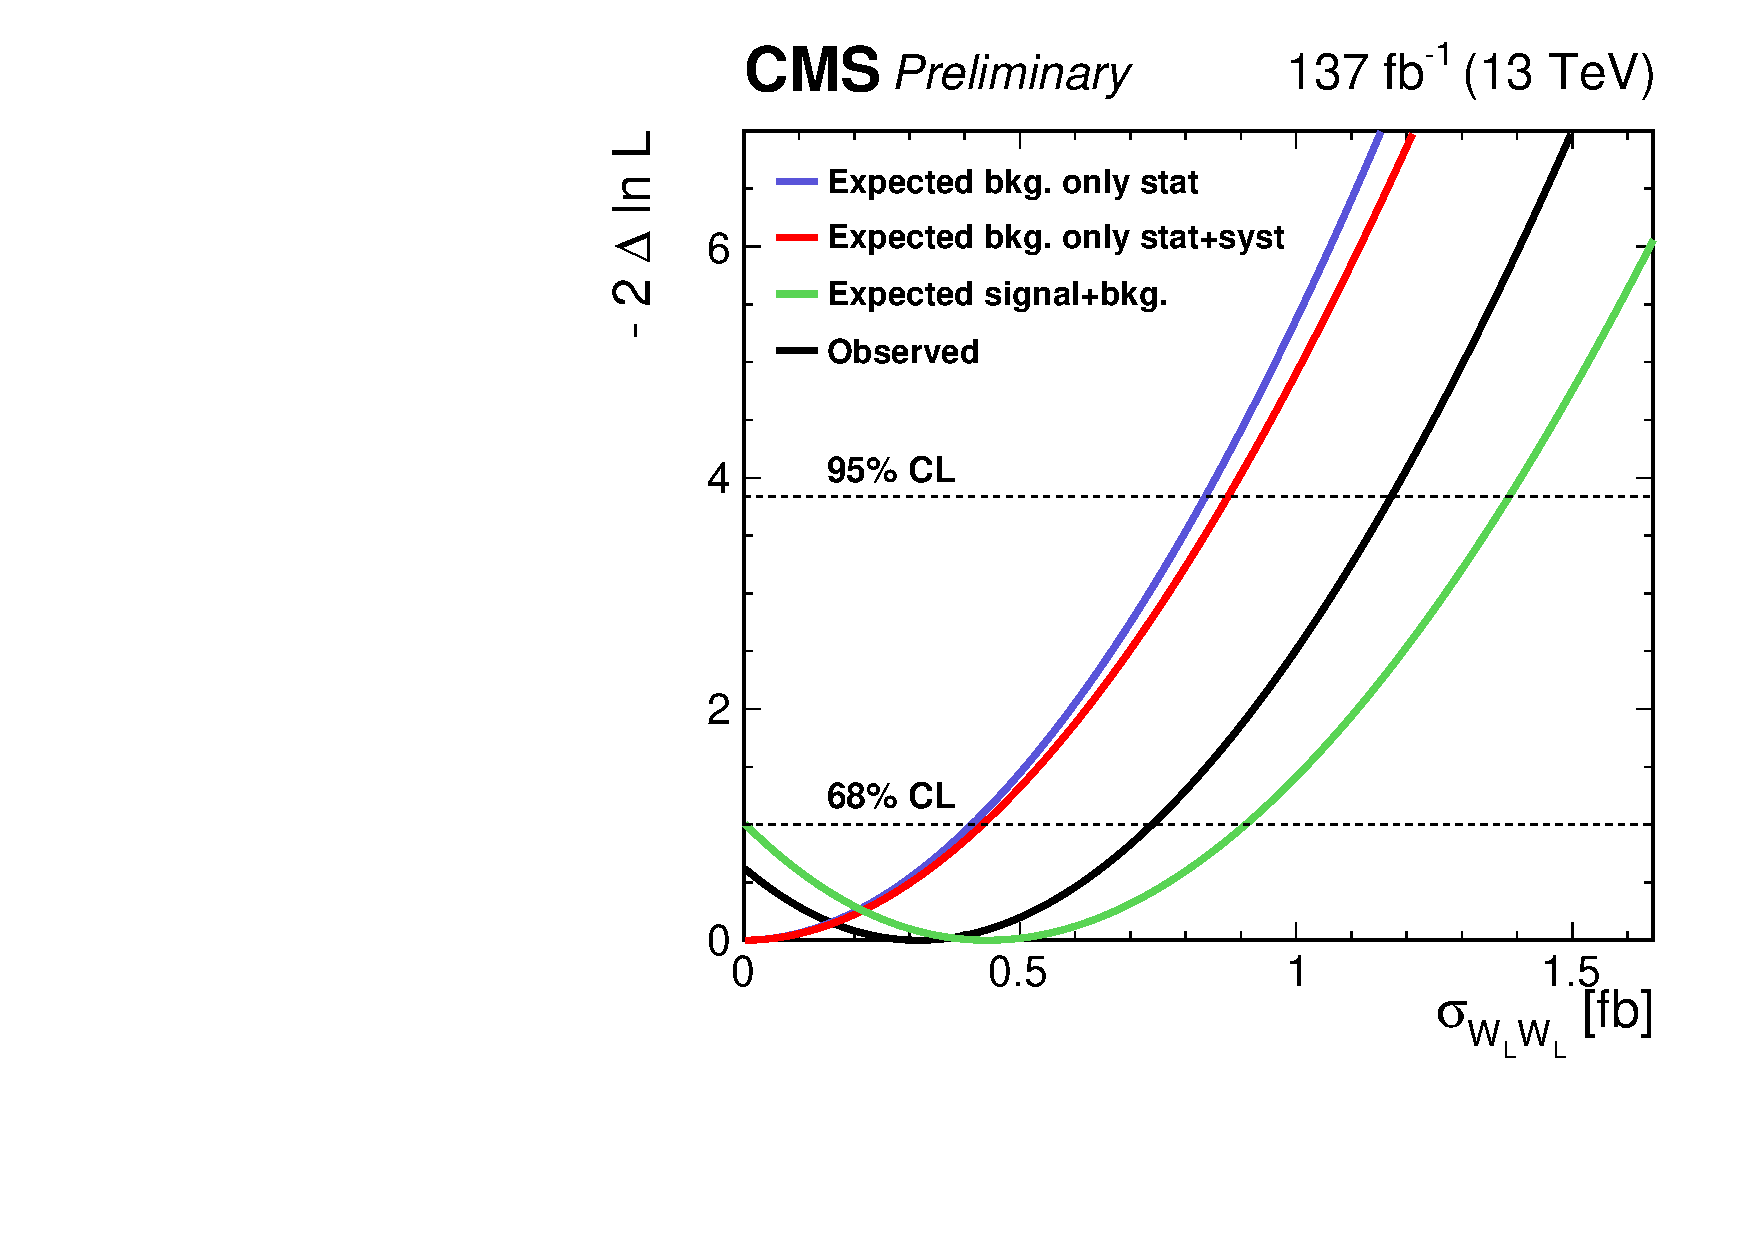
\includegraphics[width=3in]{Figure-21.pdf}
\cnenfigcaption{以$\Wboson$\textsubscript{L}$\Wboson$\textsubscript{L}截面为变量的剖面似然函数扫描. 其中红线(蓝线)代表考虑所有(只考虑统计)误差对应的零假设, 即只存在本底时的分布. 绿线为备择假设, 即存在信号和本底的预期分布. 黑线为测量结果分布}{Profile likelihood scan as a function of the $\Wboson^{\pm}$\textsubscript{L}$\Wboson^{\pm}$\textsubscript{L} cross section. The red (blue) line
represents the expected values in the background-only hypothesis considering all systematic uncertainties (only statistical uncertainties). The green line shows the expected values for the signal-plus-background hypothesis. The observed values are represented by the black line}
\label{fig:21}
\end{figure}

\section{总结与展望}

矢量玻色子散射过程可以直接验证Higgs机制, 同时也对标准模型之外的新物理极其敏感. 本文介绍了CMS实验利用一期和二期取数在矢量玻色子散射研究方面的进展, 包括, LHC上第一个被发现的矢量玻色子散射过程即同电荷W玻色子散射过程, 以及首个极化玻色子散射的测量. 目前的测量结果都表明, 数据与标准模型的预期在误差范围内是相符的. 在有效理论框架下, 这些结果导致了对四规范玻色子反常耦合的强有力的限制. 目前, 更多的分析逐步转向用所有二期数据(2016-2018)进行测量, 更多的数据量以及更先进的分析方法无疑会带来更精确的测量结果, 从而对自发电弱对称破缺作出更深入的探测, 以及在新的相空间揭示出标准模型与数据可能的偏离. 

LHC 目前处于第二次长期停机状态, 在 2022 年将进入 Run3 阶段. 此外, 在 2025-2026 年之后, LHC 将进入 HL-LHC 阶段, 为期约 10 年, 总共将收集到约 3000 fb\textsuperscript{-1} 的海量数据, 在此期间的对撞质心系能量将从 13 TeV 提升到 14 TeV. 随着 LHC 对撞能量及数据量的提升, 更高能标下的物理过程变得可以测量及得到高精度验证. 与此同时, 在 Higgs 粒子被发现之后, 高能粒子物理目前正处于关键时期: 未来方向一方面是直接寻找新物理, 比如超对称及额外维目前所给出的都是排除性质的结果; 另一方面, 随着越来越多对撞数据的累积, 对标准模型的检验在深度和广度上都得到了很大的提升.

纵向极化散射是 HL-LHC 的最重要的物理目标. VBS 过程的纵向极化部分虽然只占整体的 5-10\%, 但由于W/Z玻色子正是合并了Higgs场的Goldstone分量才变得有质量, 其纵向极化散射部分的测量将能直接检验高能散射的幺正机制, 以及探测额外的 Higgs 等新物理. 对于同号 WW 散射, 传统方法预期 HL-LHC 可以给出预期敏感度为 3-4 倍标准偏差\upcite{69,70}, 为了改进测量敏感度, 多变量方法、矩阵元方法和机器学习等近期得到广泛的应用\upcite{49}, 相比传统结果, 灵敏度有了很大的提高.

对于 VBS 和多玻色子产生过程, 利用越来越多的数据, 可进行更加精确的测量, 给出更多微分截面分布信息, 进而深入检验标准模型的自洽性, 以及间接地探索高能标的新物理. 例如, 在 ATLAS 和 CMS 之前的 VBS 分析中, 对反常规范玻色子耦合的研究大都是在量纲为8的有效理论框架下进行 \upcite{24}, 并且忽略量纲为6的有效算子, 认为后者已经在其他测量如双玻色子研究中受到很强的限制. 然而, 从 W 玻色子散射的幺正性机制可以看到, 反常规范玻色子耦合与 HVV 耦合密切相关. 随着数据量的增加以及 VBS 研究的深入开展, 在更一般性的有效场论(Effective Field Theory, EFT)框架下全局性检验标准模型的自洽性, 已经变得越来越迫切\upcite{71,72,73}.

此外, HL-LHC 的探测器升级对于改进相关结果具有重要意义. 例如高颗粒度量能器\upcite{74}和时间分辨探测器\upcite{75}, 可以有效压低 Pile-Up 效应, 提高 VBS 过程的前向喷注鉴别效率; 大快度区域扩充的径迹探测器以及触发系统的升级, 对于多玻色子末态如轻子的鉴别效率有很大的提升\upcite{76,77,78}.

%%%%%%%%%%%%%%%%%%%%%%%%%%%%%%%%%%%%%%%%%%%%%%%%%%%%%%%
%%% 致谢
%%% 非必选
%%%%%%%%%%%%%%%%%%%%%%%%%%%%%%%%%%%%%%%%%%%%%%%%%%%%%%%
\newpage
\Acknowledgements{感谢欧洲核子中心各个部门的辛勤工作以及不懈努力使得LHC维持良好的运行状态, 感谢CMS合作组来自全球各地的同事的通力合作使得CMS合作组取得了一系列的重大成果. 感谢中国国家基金委、科技部、中国科学院高能物理研究所及北京大学物理学院, 特别是核物理与核技术国家重点实验室对北大高能物理实验组的大力支持.}

%%%%%%%%%%%%%%%%%%%%%%%%%%%%%%%%%%%%%%%%%%%%%%%%%%%%%%%
%%% 补充材料说明
%%% 非必选
%%%%%%%%%%%%%%%%%%%%%%%%%%%%%%%%%%%%%%%%%%%%%%%%%%%%%%%
%\Supplements{补充材料.}

%%%%%%%%%%%%%%%%%%%%%%%%%%%%%%%%%%%%%%%%%%%%%%%%%%%%%%%
%%% 参考文献, {}为引用的标签, 数字/字母均可
%%% 文中上标引用: \upcite{1,2}
%%% 文中正常引用: \cite{1,2}
%%%%%%%%%%%%%%%%%%%%%%%%%%%%%%%%%%%%%%%%%%%%%%%%%%%%%%%
\begin{thebibliography}{99}
\bibitem{1} Brüning O S, Collier P, Lebrun P, et al. LHC design report. CERN yellow reports: Monographs. CERN, Geneva[J]. 2004
\bibitem{2} ATLAS Collaboration. Physics Performance Technical Design Report[J]. 1999
\bibitem{3} Aad G, Abat E, Abbott B, et al. Expected performance of the ATLAS experiment-detector, trigger and physics[R]. SLAC National Accelerator Lab., Menlo Park, CA (United States), 2011
\bibitem{4} Aad G, Abajyan T, Abbott B, et al. Observation of a new particle in the search for the Standard Model Higgs boson with the ATLAS detector at the LHC[J]. Physics Letters B, 2012, 716(1): 1-29
\bibitem{5} Bayatian G L, Korablev A, Soha A, et al. CMS Physics: Technical Design Report, Volume I: Detector Performance and Software[R]. CMS-TDR-008-1, 2006
\bibitem{6} CMS collaboration. CMS Physics: Technical Design Report, volume II: Physics Performance[J]. Journal of Physics G: Nuclear and Particle Physics, 2007, 34(6): 995
\bibitem{7} Chatrchyan S, Khachatryan V, Sirunyan A M, et al. Observation of a new boson at a mass of 125 GeV with the CMS experiment at the LHC[J]. Physics Letters B, 2012, 716(1): 30-61
\bibitem{8} Dittmaier S, Mariotti C, Passarino G, et al. Handbook of LHC Higgs cross sections: 2[J]. Differential Distributions, 2012, 1201.
\bibitem{63} Chatrchyan S, Khachatryan V, Sirunyan A M, et al. Observation of a new boson with mass near 125 GeV in pp collisions at $\sqrt {s}= 7$ and 8 TeV[J]. Journal of High Energy Physics, 2013, 2013(6): 81
\bibitem{64} Sirunyan A M, Tumasyan A, Adam W, et al. Measurements of properties of the Higgs boson decaying into the four-lepton final state in pp collisions at $\sqrt {s}= 13$ TeV[J]. Journal of High Energy Physics, 2017, 2017(11): 47
\bibitem{65} Sirunyan A M, Tumasyan A, Adam W, et al. Measurements of Higgs boson properties in the diphoton decay channel in proton-proton collisions at $\sqrt {s}= 13$ TeV[J]. Journal of High Energy Physics, 2018, 2018(11): 185
\bibitem{66} Sirunyan A M, Tumasyan A, Adam W, et al. Measurements of properties of the Higgs boson decaying to a W boson pair in pp collisions at $\sqrt {s}= 13$ TeV[J]. Physics letters B, 2019, 791: 96-129
\bibitem{67} Sirunyan A M, Tumasyan A, Adam W, et al. Measurement and interpretation of differential cross sections for Higgs boson production at $\sqrt {s}= 13$ TeV[J]. Physics letters B, 2019, 792: 369-396
\bibitem{9} Higgs P W. Broken symmetries, massless particles and gauge fields[J]. Phys. Lett., 1964, 12: 132-133
\bibitem{10} Englert F, Brout R. Broken symmetry and the mass of gauge vector mesons[J]. Physical Review Letters, 1964, 13(9): 321–323
\bibitem{11} Higgs P W. Broken symmetries and the masses of gauge bosons[J]. Physical Review Letters, 1964, 13(16): 508–509
\bibitem{12} Guralnik G S, Hagen C R, Kibble T W B. Global conservation laws and massless particles[J]. Physical Review Letters, 1964, 13(20): 585-587
\bibitem{13} Nambu Y. Quasi-particles and gauge invariance in the theory of superconductivity[J]. Physical Review, 1960, 117(3): 648
\bibitem{14} Goldstone J. Field theories with «Superconductor» solutions[J]. Il Nuovo Cimento (1955-1965), 1961, 19(1): 154-164
\bibitem{15} Glashow S L. Partial-symmetries of weak interactions[J]. Nuclear physics, 1961, 22(4): 579-588
\bibitem{16} Weinberg S. A model of leptons[J]. Physical Review Letters, 1967, 19(21): 1264
\bibitem{17} Salam A. Weak and electromagnetic interactions in Elementary particle theory, ed. N. Svartholm[J]. 1968: 367-377
\bibitem{18} Chatrchyan S, Khachatryan V, Sirunyan A M, et al. Observation of a new boson with mass near 125 GeV in pp collisions at $\sqrt {s}= 7$ and 8 TeV[J]. Journal of High Energy Physics, 2013, 2013(6): 81
\bibitem{19} Aad G, Abajyan T, Abbott B, et al. Evidence for the spin-0 nature of the Higgs boson using ATLAS data[J]. Physics Letters B, 2013, 726(1-3): 120-144
\bibitem{20} Barger V, Cheung K, Han T, et al. Strong W+ W+ scattering signals at pp supercolliders[J]. Physical Review D, 1990, 42(9): 3052
\bibitem{21} Szleper M. The Higgs boson and the physics of $ WW $ scattering before and after Higgs discovery[J]. arXiv preprint arXiv:1412.8367, 2014
\bibitem{22} Kazakov D I. Beyond the standard model (in search of supersymmetry)[J]. arXiv preprint hep-ph/0012288, 2000
\bibitem{23} Weinberg S. Phenomenological lagrangians[J]. Physica a, 1979, 96(1-2): 327-340
\bibitem{24} Éboli O J P, Gonzalez-Garcia M C, Mizukoshi J K. $p p \rightarrow j j e^{\pm} \mu^{\pm} \nu \nu \text { and } j j e^{\pm} \mu^{\mp} \nu \nu \text { at } \mathscr{O}\left(\alpha_{\mathrm{em}}^{6}\right) \text { and } \mathscr{O}\left(\alpha_{\mathrm{em}}^{4} \alpha_{s}^{2}\right)$ for the study of the quartic electroweak gauge boson vertex at CERN LHC[J]. Physical Review D, 2006, 74(7): 073005
\bibitem{25} Degrande C, Eboli O, Feigl B, et al. Monte Carlo tools for studies of non-standard electroweak gauge boson interactions in multi-boson processes: A Snowmass White Paper[J]. arXiv preprint arXiv:1309.7890, 2013
\bibitem{26} Khachatryan V, Sirunyan A M, Tumasyan A, et al. Measurement of the cross section for electroweak production of Z$\gamma$ in association with two jets and constraints on anomalous quartic gauge couplings in proton–proton collisions at $\sqrt{s} = 8$ TeV[J]. Physics Letters B, 2017, 770: 380-402
\bibitem{27} Sirunyan A M, Tumasyan A, Adam W, et al. Observation of electroweak production of same-sign W boson pairs in the two jet and two same-sign lepton final state in proton-proton collisions at $\sqrt{s} = 13$ TeV[J]. Physical Review Letters, 2018, 120(8): 081801
\bibitem{28} Sirunyan A M, Erbacher R, Carrillo Montoya C A, et al. Observation of electroweak production of W$\gamma $ with two jets in proton-proton collisions at $\sqrt {s}= $13 TeV[R]. CMS-SMP-19-008, CERN-EP-2020-143; arXiv: 2008.10521, 2020
\bibitem{29} Zhu B, Govoni P, Mao Y, et al. Same sign WW scattering process as a probe of Higgs boson in pp collision at $\sqrt {s}= 10$ TeV[J]. The European Physical Journal C, 2011, 71(1): 1514
\bibitem{30} Ballestrero A, Belhouari A, Bevilacqua G, et al. PHANTOM: a Monte Carlo event generator for six parton final states at high energy colliders[J]. Computer Physics Communications, 2009, 180(3): 401-417
\bibitem{31} Ballestrero A, Franzosi D B, Oggero L, et al. Vector Boson scattering at the LHC: counting experiments for unitarized models in a full six fermion approach[J]. Journal of High Energy Physics, 2012, 2012(3): 31
\bibitem{32} Ballestrero A, Maina E, Pelliccioli G. W boson polarization in vector boson scattering at the LHC[J]. Journal of High Energy Physics, 2018, 2018(3): 170
\bibitem{33} Alwall J, Frederix R, Frixione S, et al. The automated computation of tree-level and next-to-leading order differential cross sections, and their matching to parton shower simulations[J]. Journal of High Energy Physics, 2014, 2014(7): 79
\bibitem{34} Alwall J, Herquet M, Maltoni F, et al. MadGraph 5: going beyond[J]. Journal of High Energy Physics, 2011, 2011(6): 128
\bibitem{35} Frederix R, Frixione S. Merging meets matching in MC@NLO[J]. Journal of High Energy Physics, 2012, 2012(12): 61
\bibitem{36} Sjöstrand T, Mrenna S, Skands P. PYTHIA 6.4 physics and manual[J]. Journal of High Energy Physics, 2006, 2006(05): 026
\bibitem{37} Sjöstrand T, Mrenna S, Skands P. A brief introduction to PYTHIA 8.1[J]. Computer Physics Communications, 2008, 178(11): 852-867
\bibitem{38} Khachatryan V. Study of Vector Boson Scattering and Search for New Physics in Events with Two Same-Sign Leptons and Two Jets[J]. Physical Review Letters, 2015, 114(5): 051801.
\bibitem{39} Georgi H, Machacek M. Doubly charged Higgs bosons[J]. Nuclear Physics B, 1985, 262(3): 463-477
\bibitem{40} Khachatryan V, Sirunyan A M, Tumasyan A, et al. Measurement of electroweak-induced production of W$\gamma$ with two jets in pp collisions at $\sqrt {s}= 8$ TeV and constraints on anomalous quartic gauge couplings[J]. Journal of High Energy Physics, 2017, 2017(6): 106
\bibitem{41} CMS Collaboration. Performance of photon reconstruction and identification with the CMS detector in proton-proton collisions at $\sqrt {s} = 8 $ TeV[J]. Journal of Instrumentation, 2015, 10(08): P08010
\bibitem{42} CMS collaboration. Identification of b-quark jets with the CMS experiment[J]. Journal of Instrumentation, 2013, 8(04): P04013
\bibitem{43} CMS Collaboration. Identification of b quark jets at the CMS experiment in the LHC Run 2, CMS Physics Analysis Summary CMS-PAS-BTV-15-001[J]. 2016
\bibitem{44} Sirunyan A M, Tumasyan A, Adam W, et al. Measurement of the cross section for electroweak production of a Z boson, a photon and two jets in proton-proton collisions at $\sqrt {s} = 13 $ TeV and constraints on anomalous quartic couplings[J]. Journal of High Energy Physics (Online), 2020, 2020(FERMILAB-PUB-20-132-CMS; arXiv: 2002.09902; CMS-SMP-18-007; CERN-EP-2020-007)
\bibitem{45} Aarrestad T, Brzhechko D, Caminada L, et al. Measurement of electroweak WZ boson production and search for new physics in WZ+ two jets events in pp collisions at $\sqrt {s}= 13$ TeV[J]. Physics Letters B, 2019, 795: 281-307
\bibitem{46} Sirunyan A M, Tumasyan A, Adam W, et al. Measurement of vector boson scattering and constraints on anomalous quartic couplings from events with four leptons and two jets in proton–proton collisions at $\sqrt {s} = 13 $ TeV[J]. Physics letters B, 2017, 774: 682-705
\bibitem{47} Voss H, Höcker A, Stelzer J, et al. TMVA, the toolkit for multivariate data analysis with ROOT[C]//XI International Workshop on Advanced Computing and Analysis Techniques in Physics Research. SISSA Medialab, 2009, 50: 040
\bibitem{48} Campbell J M, Ellis R K. MCFM for the Tevatron and the LHC (2010) Nucl. Phys. B[J]. Proc. Suppl, 205-206
\bibitem{49} Lee J, Chanon N, Levin A, et al. Polarization fraction measurement in same-sign WW scattering using deep learning[J]. Physical Review D, 2019, 99(3): 033004
\bibitem{50} Delphes 3 Collaboration. J. de Favereau et al., DELPHES 3, A modular framework for fast simulation of a generic collider experiment[J]. JHEP, 2014, 2: 057
%\bibitem{51} Chollet F. Keras documentation[J]. Keras. io, 2015
\bibitem{52} Abadi M, Agarwal A, Barham P, et al. TensorFlow: Large-scale machine learning on heterogeneous systems[J]. 2015
\bibitem{53} Lee J, Chanon N, Levin A, et al. Polarization fraction measurement in ZZ scattering using deep learning[J]. Physical Review D, 2019, 100(11): 116010
\bibitem{54} Jolliffe I T, Cadima J. Principal component analysis: a review and recent developments[J]. Philosophical Transactions of the Royal Society A: Mathematical, Physical and Engineering Sciences, 2016, 374(2065): 20150202
\bibitem{55} CMS collaboration. Measurements of production cross sections of polarized same-sign W boson pairs in association with two jets in proton-proton collisions at $\sqrt{s} = 13$ TeV[R]. CMS-PAS-SMP-20-006, 2020
\bibitem{56} CMS collaboration. CMS luminosity measurements for the 2016 data taking period[R]. CMS-PAS-LUM-17-001, 2017
\bibitem{57} CMS collaboration. CMS luminosity measurement for the 2017 data-taking period at $\sqrt{s} = 13$ TeV[J]. CMS Physics Analysis Summary CMS-PAS-LUM-17-004, 2018
\bibitem{58} CMS Collaboration. CMS luminosity measurement for the 2018 data-taking period at $\sqrt{s} = 13$ TeV. CMS Physics Analysis Summary CMS-PAS-LUM-18-002,(2019)[J]
\bibitem{59} Franzosi D, Mattelaer O, Ruiz R, et al. Automated predictions from polarized matrix elements[J]. Journal of High Energy Physics, 2020, 2020(1912.01725): 1-46
\bibitem{60} Biedermann B, Denner A, Pellen M. Large electroweak corrections to vector-boson scattering at the Large Hadron Collider[J]. Physical Review Letters, 2017, 118(26): 261801
\bibitem{61} Biedermann B, Denner A, Pellen M. Complete NLO corrections to W$^+$ W$^+$ scattering and its irreducible background at the LHC[J]. Journal of High Energy Physics, 2017, 2017(10): 124
\bibitem{69} CMS Collaboration. Prospects for the study of vector boson scattering in same sign WW and WZ interactions at the HL-LHC with the upgraded CMS detector[J]. CMS Physics Analysis Summary CMS-PAS-SMP-14-008, 2014.
\bibitem{70} CMS Collaboration, CMS Collaboration. Study of W$^{\pm}$W$^{\pm}$ production via vector boson scattering at the HL-LHC with the upgraded CMS detector[R]. CMS-PAS-FTR-18-005, CERN, Geneva, 2018.
\bibitem{71} Grzadkowski B, Iskrzyński M, Misiak M, et al. Dimension-six terms in the Standard Model Lagrangian[J]. Journal of High Energy Physics, 2010, 2010(10): 85.
\bibitem{72} Hartland N P, Maltoni F, Nocera E R, et al. A Monte Carlo global analysis of the Standard Model Effective Field Theory: the top quark sector[J]. Journal of High Energy Physics, 2019, 2019(4): 100.
\bibitem{73} Degrande C, Fuks B, Mawatari K, et al. Electroweak Higgs boson production in the standard model effective field theory beyond leading order in QCD[J]. The European Physical Journal C, 2017, 77(4): 262.
\bibitem{74} CMS Collaboration. The phase-2 upgrade of the CMS endcap calorimeter[R]. CMS Technical Design Report, CERN-LHCC-2017-023, CMS-TDR-019, 2017.
\bibitem{75} CMS Collaboration. A MIP Timing Detector for the CMS Phase-2 Upgrade[R]. CMS Technical Design Report, CERN-LHCC-2019-003, CMS-TDR-020, 2019.
\bibitem{76} Apollinari G, Béjar Alonso I, Brüning O, et al. High-Luminosity Large Hadron Collider (HL-LHC): Technical Design Report V. 0.1[R]. CERN Yellow Reports: Monographs. CERN, Geneva, 2017[J].
\bibitem{77} CMS collaboration. Technical proposal for the phase-II upgrade of the CMS detector[J]. CMS Technical proposal CERN-LHCC-2015-010, CMS-TDR-15-02, CERN, 2015.
\bibitem{78} ATLAS and CMS Collaborations. Report on the Physics at the HL-LHC and Perspectives for the HE-LHC[R]. CERN-LPCC-2019-01, CMS-FTR-19-001, ATL-PHYS-PUB-2019-006, 2019.

\end{thebibliography}

%%%%%%%%%%%%%%%%%%%%%%%%%%%%%%%%%%%%%%%%%%%%%%%%%%%%%%%
%%% 附录章节, 自动从A编号, 以\section开始一节
%%% 非必选
%%%%%%%%%%%%%%%%%%%%%%%%%%%%%%%%%%%%%%%%%%%%%%%%%%%%%%%
%\begin{appendix}
%\section{附录}
%附录从这里开始.
%\begin{figure}[H]
%\centering
%%\includegraphics{fig1.eps}
%\cnenfigcaption{附录里的图}{Caption}
%\label{fig1}
%\end{figure}
%\end{appendix}


%%%%%%%%%%%%%%%%%%%%%%%%%%%%%%%%%%%%%%%%%%%%%%%%%%%%%%%
%%% 自动生成英文标题部分
%%%%%%%%%%%%%%%%%%%%%%%%%%%%%%%%%%%%%%%%%%%%%%%%%%%%%%%
\newpage
\makeentitle


%%%%%%%%%%%%%%%%%%%%%%%%%%%%%%%%%%%%%%%%%%%%%%%%%%%%%%%
%%% 主要作者英文简介, 数量不超过4个
%%% \authorcv[zp1.eps]{Ming XING}{was born in ...}
%%% [照片文件名]请提供清晰的一寸浅色背景照片, 宽高比为 25:35
%%% {姓名}与英文标题处一致
%%%%%%%%%%%%%%%%%%%%%%%%%%%%%%%%%%%%%%%%%%%%%%%%%%%%%%%
%\authorcv[]{Ming XING}{was born in ...}

%\authorcv[]{Ming XING}{was born in ...}

%\vspace*{6mm} % 调整照片行间距

%\authorcv[]{Ming XING}{was born in ...}

%\authorcv[]{Ming XING}{was born in ...}



%%%%%%%%%%%%%%%%%%%%%%%%%%%%%%%%%%%%%%%%%%%%%%%%%%%%%%%
%%% 补充材料, 以附件形式作网络在线, 不出现在印刷版中
%%% 不做加工和排版, 仅用于获得图片和表格编号
%%% 自动从I编号, 以\section开始一节
%%% 可以没有\section
%%%%%%%%%%%%%%%%%%%%%%%%%%%%%%%%%%%%%%%%%%%%%%%%%%%%%%%
%\begin{supplement}
%\section{supplement1}
%自动从I编号, 以section开始一节.
%\begin{figure}[H]
%\centering
%\includegraphics{fig1.eps}
%\cnenfigcaption{补充材料里的图}{Caption}
%\label{fig1}
%\end{figure}
%\end{supplement}

\end{document}


%%%%%%%%%%%%%%%%%%%%%%%%%%%%%%%%%%%%%%%%%%%%%%%%%%%%%%%
%%% 本模板使用的latex排版示例
%%%%%%%%%%%%%%%%%%%%%%%%%%%%%%%%%%%%%%%%%%%%%%%%%%%%%%%

%%% 章节
\section{}
\subsection{}
\subsubsection{}


%%% 普通列表
\begin{itemize}
\item Aaa aaa.
\item Bbb bbb.
\item Ccc ccc.
\end{itemize}

%%% 自由编号列表
\begin{itemize}
\itemindent 4em
\item[(1)] Aaa aaa.
\item[(2)] Bbb bbb.
\item[(3)] Ccc ccc.
\end{itemize}

%%% 定义、定理、引理、推论等, 可用下列标签
%%% definition 定义
%%% theorem 定理
%%% lemma 引理
%%% corollary 推论
%%% axiom 公理
%%% propsition 命题
%%% example 例
%%% exercise 习题
%%% solution 解名
%%% notation 注
%%% assumption 假设
%%% remark 注释
%%% property 性质
%%% []中的名称可以省略, \label{引用名}可在正文中引用
\begin{definition}[定义名]\label{def1}
定义内容.
\end{definition}



%%% 单图
%%% 可在文中使用图\ref{fig1}引用图编号
\begin{figure}[!t]
\centering
\includegraphics{fig1.eps}
\cnenfigcaption{中文图题}{Caption}
\label{fig1}
\end{figure}

%%% 并排图
%%% 可在文中使用图\ref{fig1}、图\ref{fig2}引用图编号
\begin{figure}[!t]
\centering
\begin{minipage}[c]{0.48\textwidth}
\centering
\includegraphics{fig1.eps}
\end{minipage}
\hspace{0.02\textwidth}
\begin{minipage}[c]{0.48\textwidth}
\centering
\includegraphics{fig2.eps}
\end{minipage}\\[3mm]
\begin{minipage}[t]{0.48\textwidth}
\centering
\cnenfigcaption{中文图题1}{Caption1}
\label{fig1}
\end{minipage}
\hspace{0.02\textwidth}
\begin{minipage}[t]{0.48\textwidth}
\centering
\cnenfigcaption{中文图题2}{Caption2}
\label{fig2}
\end{minipage}
\end{figure}

%%% 并排子图
%%% 需要英文分图题 (a)...; (b)...
\begin{figure}[!t]
\centering
\begin{minipage}[c]{0.48\textwidth}
\centering
\includegraphics{subfig1.eps}
\end{minipage}
\hspace{0.02\textwidth}
\begin{minipage}[c]{0.48\textwidth}
\centering
\includegraphics{subfig2.eps}
\end{minipage}
\cnenfigcaption{中文图题}{Caption}
\label{fig1}
\end{figure}

%%% 算法
%%% 可在文中使用 算法\ref{alg1} 引用算法编号
\begin{algorithm}
%\floatname{algorithm}{Algorithm}%更改算法前缀名称
%\renewcommand{\algorithmicrequire}{\textbf{Input:}}% 更改输入名称
%\renewcommand{\algorithmicensure}{\textbf{Output:}}% 更改输出名称
\footnotesize
\caption{算法标题}
\label{alg1}
\begin{algorithmic}[1]
    \REQUIRE $n \geq 0 \vee x \neq 0$;
    \ENSURE $y = x^n$;
    \STATE $y \Leftarrow 1$;
    \IF{$n < 0$}
        \STATE $X \Leftarrow 1 / x$;
        \STATE $N \Leftarrow -n$;
    \ELSE
        \STATE $X \Leftarrow x$;
        \STATE $N \Leftarrow n$;
    \ENDIF
    \WHILE{$N \neq 0$}
        \IF{$N$ is even}
            \STATE $X \Leftarrow X \times X$;
            \STATE $N \Leftarrow N / 2$;
        \ELSE[$N$ is odd]
            \STATE $y \Leftarrow y \times X$;
            \STATE $N \Leftarrow N - 1$;
        \ENDIF
    \ENDWHILE
\end{algorithmic}
\end{algorithm}

%%% 简单表格
%%% 可在文中使用 表\ref{tab1} 引用表编号
\begin{table}[!t]
\cnentablecaption{表题}{Caption}
\label{tab1}
\footnotesize
\tabcolsep 49pt %space between two columns. 用于调整列间距
\begin{tabular*}{\textwidth}{cccc}
\toprule
  Title a & Title b & Title c & Title d \\\hline
  Aaa & Bbb & Ccc & Ddd\\
  Aaa & Bbb & Ccc & Ddd\\
  Aaa & Bbb & Ccc & Ddd\\
\bottomrule
\end{tabular*}
\end{table}

%%% 换行表格
\begin{table}[!t]
\cnentablecaption{表题}{Caption}
\label{tab1}
\footnotesize
\def\tabblank{\hspace*{10mm}} %blank leaving of both side of the table. 左右两边的留白
\begin{tabularx}{\textwidth} %using p{?mm} to define the width of a column. 用p{?mm}控制列宽
{@{\tabblank}@{\extracolsep{\fill}}cccp{100mm}@{\tabblank}}
\toprule
  Title a & Title b & Title c & Title d \\\hline
  Aaa & Bbb & Ccc & Ddd ddd ddd ddd.

  Ddd ddd ddd ddd ddd ddd ddd ddd ddd ddd ddd ddd ddd ddd ddd ddd ddd ddd ddd ddd ddd ddd ddd ddd ddd ddd ddd ddd ddd ddd ddd.\\
  Aaa & Bbb & Ccc & Ddd ddd ddd ddd.\\
  Aaa & Bbb & Ccc & Ddd ddd ddd ddd.\\
\bottomrule
\end{tabularx}
\end{table}

%%% 单行公式
%%% 可在文中使用 (\ref{eq1})式 引用公式编号
%%% 如果是句子开头, 使用 公式(\ref{eq1}) 引用
\begin{equation}
A(d,f)=d^{l}a^{d}(f),
\label{eq1}
\end{equation}

%%% 不编号的单行公式
\begin{equation}
\nonumber
A(d,f)=d^{l}a^{d}(f),
\end{equation}

%%% 公式组
\begin{eqnarray}
\nonumber
&X=[x_{11},x_{12},\ldots,x_{ij},\ldots ,x_{n-1,n}]^{\rm T},\\
\nonumber
&\varepsilon=[e_{11},e_{12},\ldots ,e_{ij},\ldots ,e_{n-1,n}],\\
\nonumber
&T=[t_{11},t_{12},\ldots ,t_{ij},\ldots ,t_{n-1,n}].
\end{eqnarray}

%%% 条件公式
\begin{eqnarray}
\sum_{j=1}^{n}x_{ij}-\sum_{k=1}^{n}x_{ki}=
\left\{
\begin{aligned}
1,&\quad i=1,\\
0,&\quad i=2,\ldots ,n-1,\\
-1,&\quad i=n.
\end{aligned}
\right.
\label{eq1}
\end{eqnarray}

%%% 其他格式
\footnote{Comments.} %footnote. 脚注
\raisebox{-1pt}[0mm][0mm]{xxxx} %put xxxx upper or lower. 控制xxxx的垂直位置

%%% 图说撑满
\Caption\protect\linebreak \leftline{Caption}
